% 美赛模板:正文部分

\documentclass[12pt]{article}  % 官方要求字号不小于 12 号,此处选择 12 号字体
% \linespread{1.1}
% \bibliographystyle{plain}
% 本模板不需要填写年份,以当前电脑时间自动生成
% 请在以下的方括号中填写队伍控制号
\usepackage[048]{easymcm}  % 载入 EasyMCM 模板文件
\problem{2}  % 请在此处填写题号
% \usepackage{mathptmx}  % 这是 Times 字体,中规中矩 
\usepackage{palatino}  % mathpazo 这palatino是 COMAP 官方杂志采用的更好看的 Palatino 字体,可替代以上的 mathptmx 宏包
\usepackage{pdfpages}
\usepackage{longtable}
\usepackage{tabu}
\usepackage{threeparttable}
\usepackage{listings}
\usepackage{paralist}
\let\itemize\compactitem
\let\enditemize\endcompactitem
% \let\enumerate\compactenum
% \let\endenumerate\endcompactenum
% \let\description\compactdesc
% \let\enddescription\endcompactdesc
% \usepackage{biblatex} 
% \usepackage{cite}
% \usepackage{natbib}
\newcommand{\upcite}[1]{\textsuperscript{\textsuperscript{\cite{#1}}}}
\title{How the Revolution in Music Happened}  % 标题

% 如需要修改题头(默认为 MCM/ICM),请使用以下命令(此处修改为 MCM)
%\renewcommand{\contest}{ICM}

% 文档开始
\begin{document}
	
	% 此处填写摘要内容
	\begin{abstract}
		
		% (Need to be reviewed)
		"Take a sad song and make it better.", sung \textit{the Beatles}, who left a strong mark in the history of music. In this paper, we deeply explore the magic of music - its influence network, evolution path, and effects on the culture.
		
		In \textsc{Task 1}, we build a \textit{directed network} between influencers and followers. Based on \textit{network theory}, we proposed three different metrics - Degree Centrality, Weighted Degree Centrality and Eigen Centrality. Then we develop a combination of these metrics as a comprehensive measure of music influence. After that, we create a subnetwork to illustrate our influence measure.
		
		In \textsc{Task 2}, we first preprocess the data using \textit{Principal Component Analysis} to reduce dimension and collinearity. Then we define and calculate the distance between different tracks to obtain the similarity between artists. By calculating the average similarity, we apply \textit{Mann-Whitney U test}. Results show that with the probability of 62.8\% and $\mathtt{P-Value} < 0.001$, artists within a genre are more similar than those between genres.
		
		In \textsc{Task 3}, we find that similarities and influences within and between genres differ greatly. To distinguish one genre from others, we build a \textit{Genre Classification Tree Model}. By analysing the number of influencers in different period, we explore the evolution path of genres. Based on the \textit{directed network} on genre scale, we find Pop/Rock has a strong relationship with R\&B, Blues and Folk.
		
		In \textsc{Task 4}, we first still use the $ sim_{ij} $ defined in \textsc{Task 2} to find and rank the degree of similarity between the influencers and the influenced. After that we randomly select from the key features and thus compose different combinations of features to recalculate the similarity between the influencers and the influenced. After random sampling, we rank the different combinations to compare which features are the most contagious. 
		
		In \textsc{Task 5}, we first analyze the rise and decline of genres and find the music revolution in 1950s. We proposed a \textit{Dynamic Programming Algorithm} to detect change points in music characteristics which are consistent with the revolution. Our results show that acousticness, energy, danceability and loudness might signify revolutions.
		
		In \textsc{Task 6}, to get a further insight into the evolution in Pop/Rock, we propose an \textit{Dynamic Influencer Indicator} based on the lagging trend in music characteristics of the whole genre. From 1960s to 2010s, there are 10 dynamic influencers, each has his/her unique influence on the genre. Moreover, we explain the evolution of Pop/Rock.
		
		In \textsc{Task 7}, three important periods are detected based on \textit{Time-Series Analysis}, which show the cultural influence of music. Based on the model established, we identify social changes like countercultural movement and technological changes such as the proliferation of the Internet.
		
		Finally, we conduct sensitivity analysis, which shows the robustness of our model. We also summerize the stengths and weaknesses and provide insights to ICM society about the evolution and cultural influence of music.
		
		
		
		
		% Here is the abstract of your paper.
		
		% Firstly, that is ...
		
		% Secondly, that is ...
		
		% Finally, that is ...
		
		% 美赛论文中无需注明关键字。若您一定要使用,
		% 请将以下两行的注释号 '%' 去除,以使其生效
		\vspace{5pt}
		\textbf{Keywords}: Directed Network, Random Sampling, Dynamic Planning, Change Points Analysis
		
	\end{abstract}
	
	\maketitle % 生成 Summary Sheet
	
	\tableofcontents  % 生成目录
	
	
	% 正文开始
	% Chapter 1: Introduction
	\section{Introduction}
	
	\subsection{Problem Background}
	
	Nowadays, various kinds of music has increasingly become an indispensable part of human life. Thousands of artists influence each other and form a complex music influence network. While some genres show great similarity to each other, other genres are quite different in music characteristics. Some artists are passionate revolutionaries, who lead to an emergence of a new genre or reinvention of an existing genre. Despite of cultural influence, the change of artists' musical characteristics also indicate external events like the Hippie Movement and the proliferation of Internet. ln order to further explore the music influence network and the role music has played on the society, ICM require us to do:
	
	\begin{itemize}
		\setlength{\parsep}{0ex} %段落间距
		\setlength{\topsep}{2ex} %列表到上下文的垂直距离
		\setlength{\itemsep}{1ex} %条目间距
		\item Build a complex network between influencers and followers based on dataset "influnce\_data.csv" and develop metrics to capture the musical influence in the network. 
		\item Use various musical characteristics in dataset "full\_music\_data.csv" to measure music similarity and judge whether musicians in the same genre are more similar than those in different genres.
		\item Compare similarities and influences between and within genres.
		\item Get a further insight into the similarity of music characters between influencers and followers.
		\item Identify the characteristics and major artists that signify music evolution. 
		\item Develop indicators to analyse dynamic influencers and corresponding influence processes of musical evolution in one genre.
		\item Identify the effects of social, political, or technological changes within the network and find the cultural influence of music. 
	\end{itemize}
	
	
	
	\subsection{Our work}
	
	\begin{enumerate}[\bfseries 1.]
		\setlength{\parsep}{0ex} %段落间距
		\setlength{\topsep}{2ex} %列表到上下文的垂直距离
		\setlength{\itemsep}{1ex} %条目间距
		\item The key to this problem is to define directed influencer network and propose metrics that comprehensively measure the music influence of each influencers in the network.
		\item It is of great essence to define the distance between music works of artists, from which we can obtain the similarities between artists.
		\item lt is necessary to define the distance between genres and measure similarities between them. We plan to build a classification tree to distinguish one genre from others. Besides, we can show how genres changing over time and the relationship between genres using visualization.
		\item We continue to use the variables defined in Task2 to produce different results with the help of random sampling, then comparing the most "contagious" characteristics.
		\item To handle this problem, we propose a \textit{Change Point Detection} model based on \textit{DP algorithm} and match the change of music characters with the musical revolution.
		\item In this problem, we will focus on Pop/Rock and then discuss the major contributors to the Pop/Rock evolution through decades.
		\item Based on \textit{time series analysis}, we intend to find the connection between the change in music characteristics and the external events. We also detect several cultural influence of music in different time or circumstances.
		
	\end{enumerate}
	
	\begin{figure}[htbp]
		\centering
		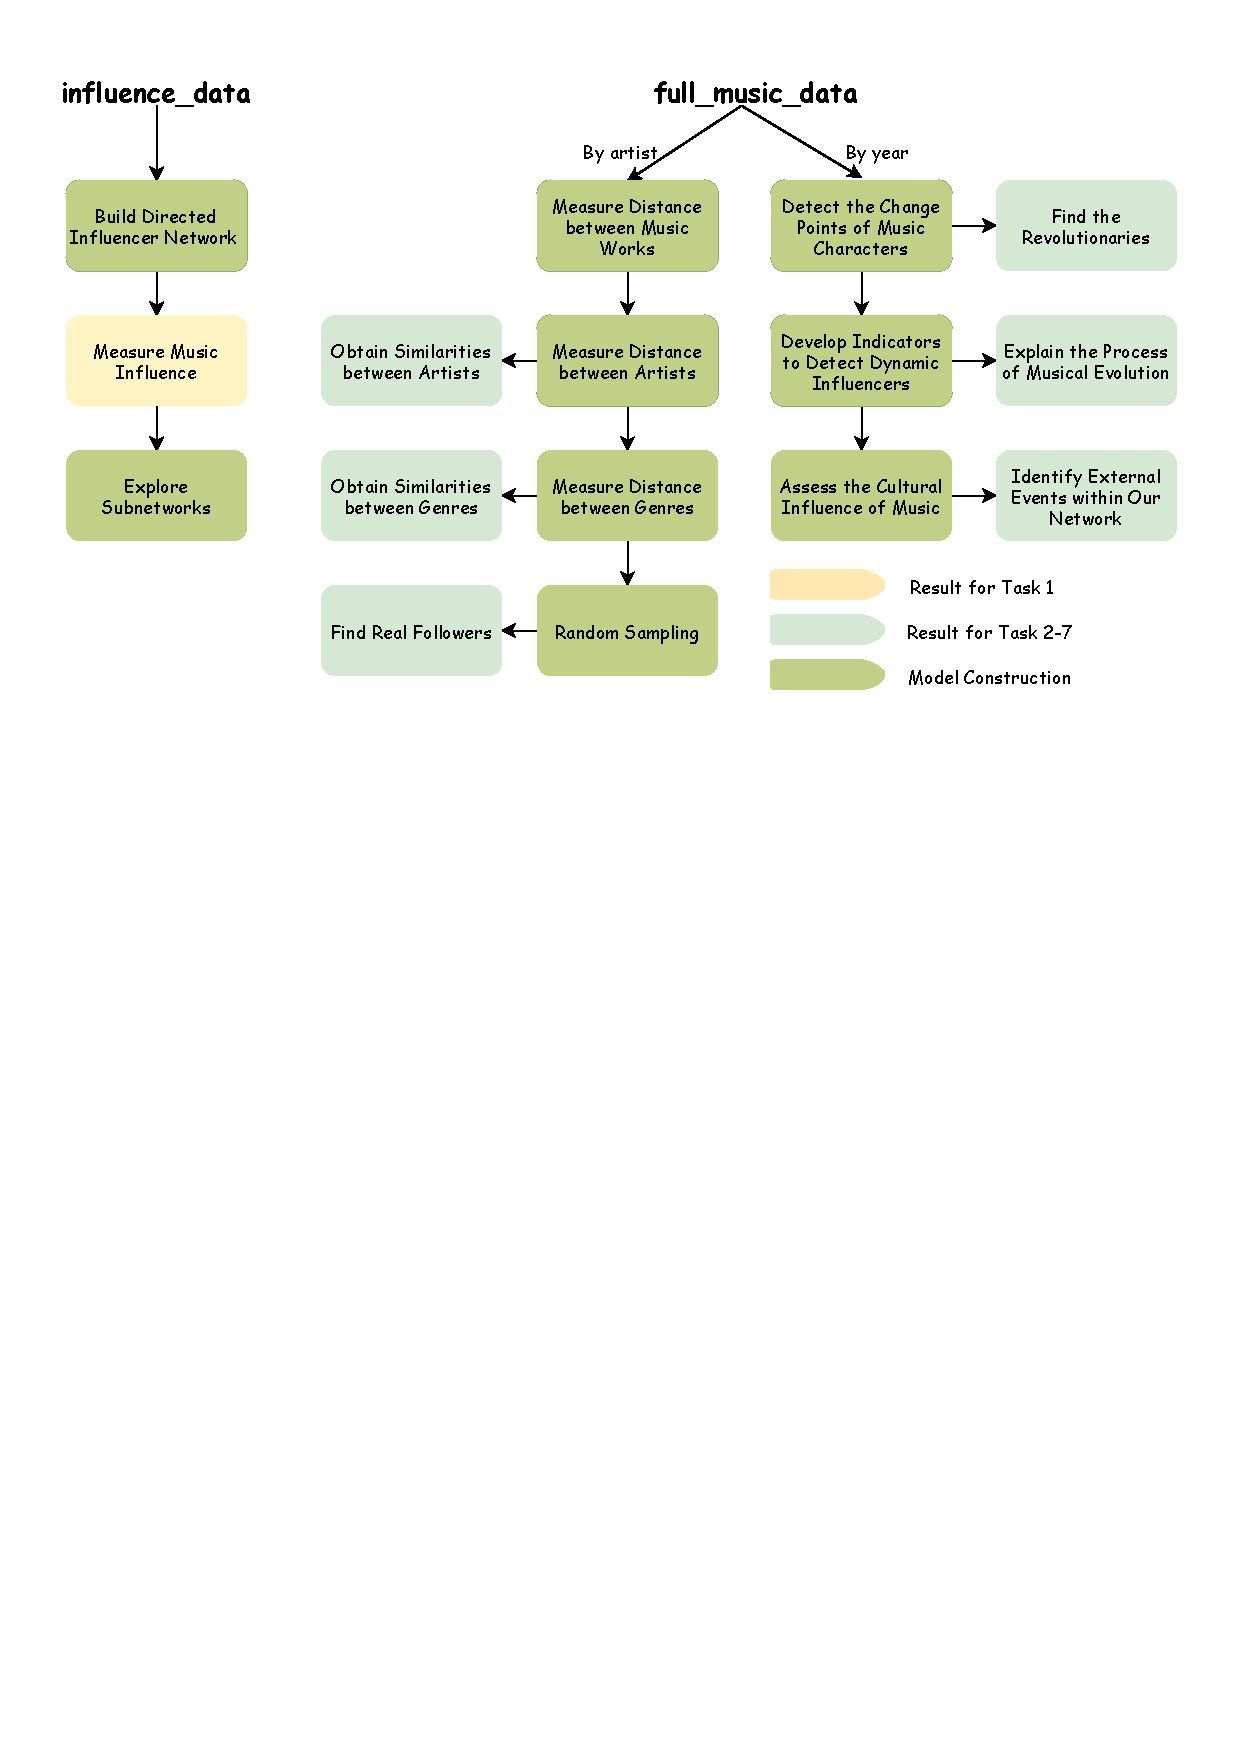
\includegraphics[width=1\textwidth]{workflow2.pdf} 	% 图片相对位置
		\caption{Workflow of our paper}		% 图片标题 
		\label{fig:exam_network}							% 图片标签
	\end{figure}
	% \section{Introduction}
	% \subsection{Problem Background}
	% Here is the problem background ...
	
	% Two major problems are discussed in this paper, which are:
	% \begin{itemize}
		%     \item Doing the first thing.
		%     \item Doing the second thing.
		% \end{itemize}
	
	% \subsection{Literature Review}
	% A literatrue\cite{1} say something about this problem ...
	
	% \subsection{Our work}
	% We do such things ...
	
	% \begin{enumerate}[\bfseries 1.]
		%     \item We do ...
		%     \item We do ...
		%     \item We do ...
		% \end{enumerate}
	
	% Chapter 2: 模型准备
	\section{Preparation of the Models}
	\subsection{Assumptions and Justifications}
	\begin{itemize}
		\setlength{\parsep}{0ex} %段落间距
		\setlength{\topsep}{2ex} %列表到上下文的垂直距离
		\setlength{\itemsep}{1ex} %条目间距
		\item \textbf{The similarity of artists is represented by the similarity of their musical characteristics.} In all available datasets, the most reliable source of information about an artist's characteristics is tracks he/she released. Therefore, it is reasonable to use musical characteristics to represent the characteristics of artists.
		\item  \textbf{The reinvention and revolution of exisiting genre can be can be signified by the sharp change in music characteristics.} Revolution shifts in a genre will definitely change the
		music characteristics, thus we can capture revolutions based on these changes. 
		\item \textbf{In different stages of genre development, music characters changed with a linear trend over time.} This assumption is a reasonable simplification to make breakpoints identification possible. 
	\end{itemize}
	
	
	\subsection{Notations}
	The primary notations used in this paper are listed in Table \ref{tb:notation}.
	\begin{table}[!htbp]
		\begin{center}
			\caption{Notations}
			\begin{tabular}{c|l}
				\toprule
				\multicolumn{1}{m{3cm}}{\centering Symbol}
				&\multicolumn{1}{m{8cm}}{ Definition}\\
				\midrule
				$DC_{i}$& the local influence Degree Centrality of $i$th influencer \\
				$WDC_{i}$& Weighted Degree Centrality for $i$th influencer \\
				$EC_{i}$& Eigen Centrality for $i$th influencer\\
				$F-Score_{i}$& the comprehensive score of $i$th influencer \\
				$Sim_{i,j}$ & music Similarity between track $i$ and track $j$ \\
				$Acv_{i,j}$& absolute coefficient of variation of music character $j$ in genre $i$\\
				$\rho_{AB}$ & similarity score between artist A and artist B\\
				$\mu$ & length of lagging year\\
				\bottomrule
			\end{tabular}\label{tb:notation}
		\end{center}
	\end{table}
	
	
	% % Chapter 3:其他假设
	% \section{Assumptions and Justifications}
	% First and foremost, we make some basic assumptions about dragons and explain their rationales.
	% \begin{enumerate}[\bfseries \text{Assumption} 1 ]
		%     \item \textit{They continue to grow throughout their life depending on the conditions and amount of food available to them.} 
		%     \item \textit{Dragons are able to fly great distances, breath fire.}
		%     \item \textit{During the time scale we discuss in this paper, the earth's ecological environment keeps stable.}
		
		%     In our model, we don't consider the incidents that may cause great climate changes such as meteorite impacts or frequent volcanoes, since their probabilities are small.
		%     \item \textit{During the time scale we discuss in this paper, a dragon's body function won't change as the dragon grows old.}
		
		%     \item \textit{Dragons are at the top of the food chain.}
		
		%     Considering the power of dragons, the dragons can have influence on all living beings in the ecosystem while few living beings can compete with the dragon.
		%     \item \textit{Dragon's body function won't change when it is hurt.}
		
		%     Dragons can resist tremendous trauma.
		%     \item \textit{There is a upper bound for dragon's body size.}
		
		%        With the limitation of gravity and biological structure, the body size of a dragon cannot     infinitely increase.
		
		% \end{enumerate}
	
	% Then, we will make some useful assumptions in the tasks to perfect the problems.
	% \begin{enumerate}[\bfseries 1.]
		% \item The living area of the dragon is related to the quantity, intimacy, and the average weight of the dragon.
		% \item the growth rate parameter of the dragon
		% increases with the increase of the weight of the food.
		% \item Dragon survives in an ideal environment and is not affected by human activities.
		% \item Dragon's body state is similar to that of flying
		% creatures.
		% \end{enumerate}
	
	% Below, we next explore dragon characteristics, behavior, habits, diet, and interaction with their environment. Based on the additional assumptions mentioned above, four major tasks have yet to be addressed (see \textbf{Figure \ref{fig:tasks}}).
	
	% \clearpage
	\section{\textsc{Task 1: }Influencer Network Model}
	\subsection{Directed Influencer Network}
	
	We consider influencers and followers as nodes and collect all musicians together to make up the set $V = {\{v_{i}\}}^n_{i=1}$. If artist $i$ has an influence on artist $j$, then an edge from node $i$ to node $j$ will be generated. All the edges make up the set $E = {\{e_{j}\}}^m_{j=1}$, and the edges from node $i$ make up set $N(i)$. Based on the dataset "influnce\_data.csv", we build a complex network involving $n=5603\quad nodes(artists)$ and $m=42770\quad edges(influence)$ in total, as shown in \textbf{Figure \ref{fig:in_network}}
	
	\begin{figure}[htbp]
		\centering
		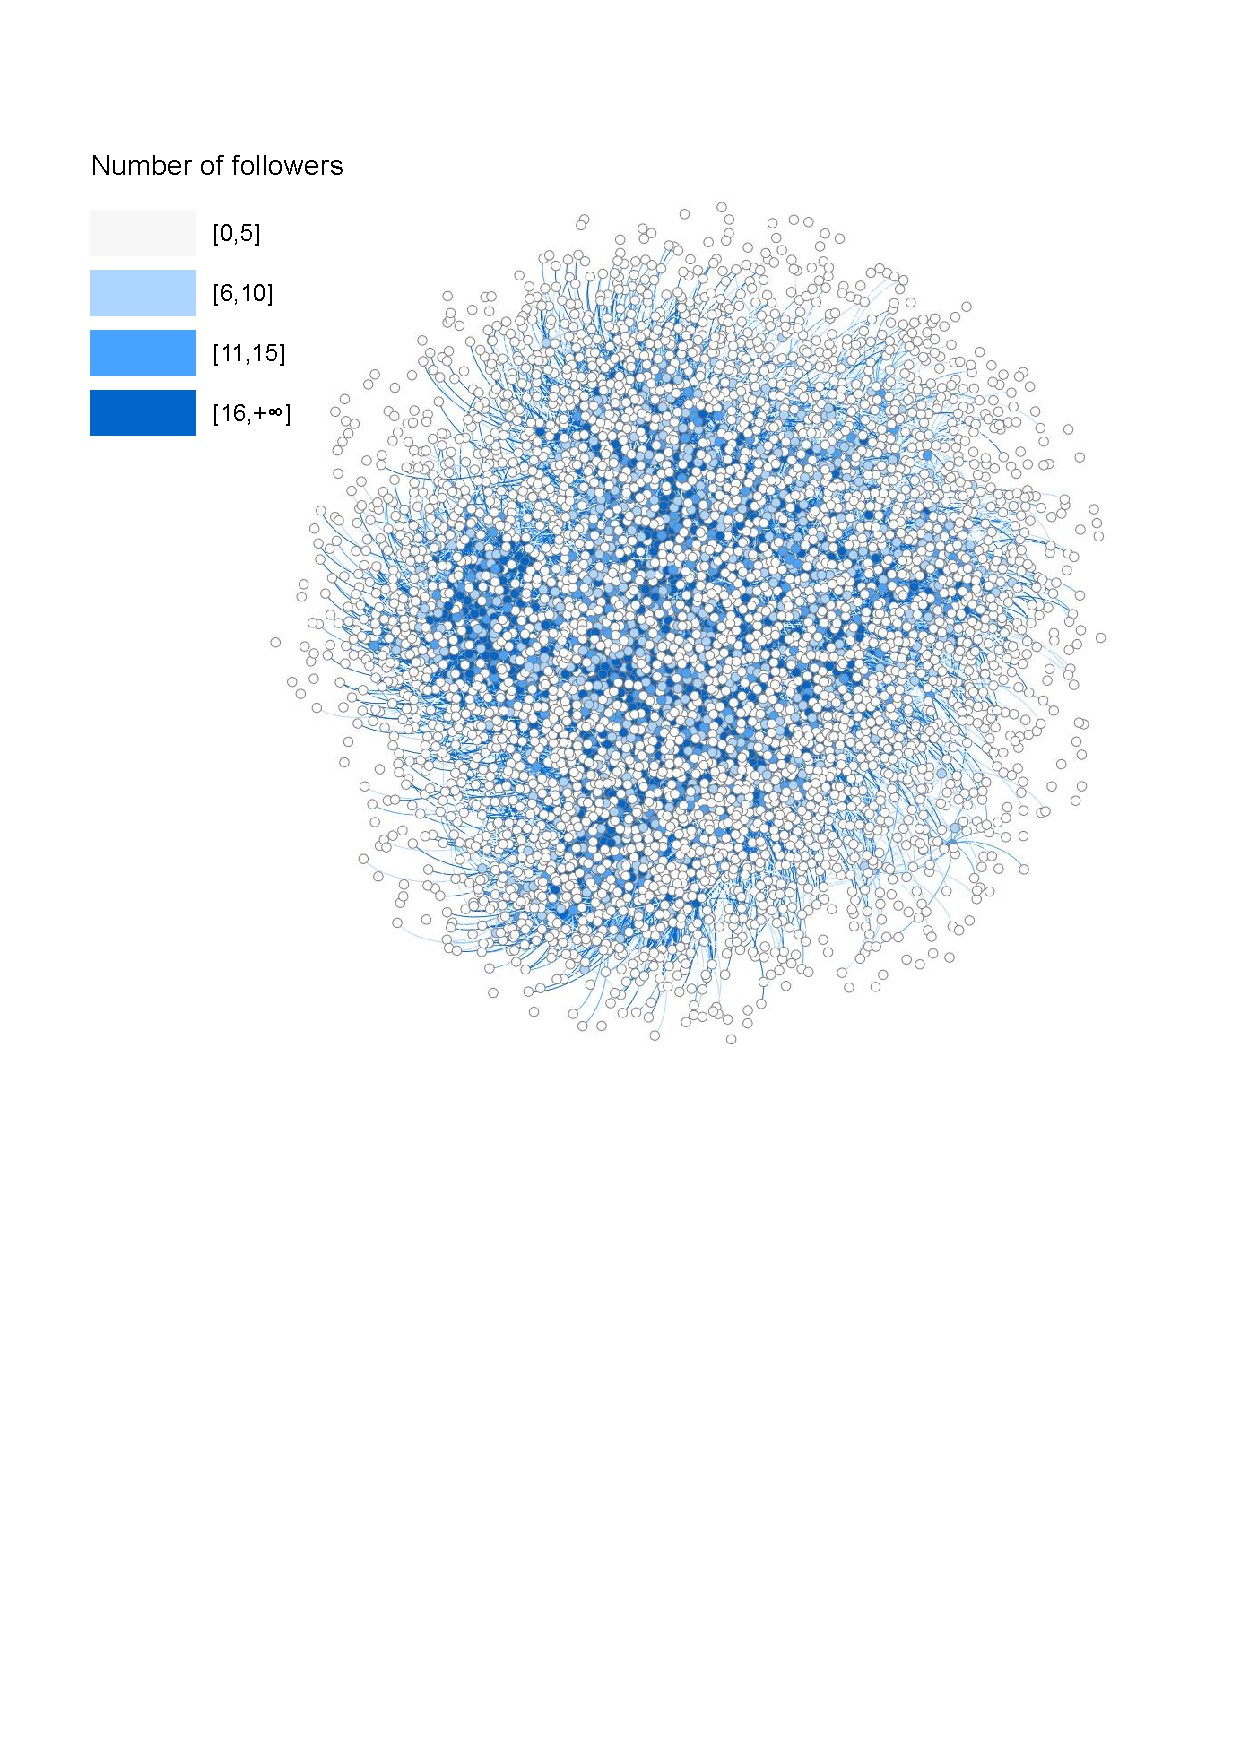
\includegraphics[width=0.65\textwidth]{Directed_Influencer_Network3 .pdf} 	% 图片相对位置
		\caption{3D Directed Influencer Network}		% 图片标题 
		\label{fig:in_network}							% 图片标签
	\end{figure}
	
	\subsection{Music Influence Measure}
	
	We now define some essential metrics to measure the music influence in the network.
	
	\begin{itemize}
		\item \textbf{Degree Centrality} 
	\end{itemize}
	
	Degree is an important concept in network theory. In directed graph, out degree of node $ v $ represents the number of edges from node $ v $[1].
	
	\begin{equation}\label{eq:outdegree}
		outdegree_v=\# N(v)
	\end{equation}
	
	A naive idea to measure the local importance of the node is the out degree of the node. In other words, we use the number of followers to measure the local influence of a musician. We call the local influence Degree Centrality and define the Degree Centrality of influencer $ i $ as follows:
	
	\begin{equation}\label{eq:outegree}
		DC_i=\frac{outdegree_i}{n}	
	\end{equation}
	
	Where $ n $ is the number of nodes in the network.
	
	\begin{itemize}
		\item  \textbf{Weighted Degree Centrality}
	\end{itemize}
	
	Some genres interact with each other closely, while others seem to have little connection. As a result, we can’t treat all the influences equally, and the edges of the network should share different weights. If a musician has an influence on artists of other genres, it means that the musician has a wide range of influence. Similarly, if a musician has an influence on future musical generations decades later, it indicates that the influence lasts for a long time. In the cases above, we align greater weight. 
	
	We define the genre of musician $ i $ as $ G(i) $. The \textit{yeargap} between followers and influencers is defined as the time difference between the start of their careers. When the \textit{yeargap} exceeds the \textit{threshold}, we call it long-time influence, otherwise short-time influence. Here we set the $ \textit{threshold} = 20$. 
	
	The weight matrix$  W = (W_{ij}) $ is defined by integrating influence range and influence duration as follows:
	
	\begin{equation}\label{eq:wij}
		W_{i j}=\left\{\begin{array}{cc}
			\frac{1}{3} *\left(1+I_{\{S(i) \neq S(j)\}}+I_{\{\textit {yeargap }>\textit { threshold }\}}\right), & j \in N(i) \\
			0, & \textit { else }
		\end{array}\right.
	\end{equation}
	
	Then we propose the Weighted Degree Centrality (WDC) to modify the Degree Centrality above:
	
	\begin{equation}\label{eq:wdci}
		WDC_{i}=\frac{1}{n} *\left\langle W_{i}, 1_{n}\right\rangle
	\end{equation}
	Where $ W_{i} $ represent the $ i $th row of matrix W, $ 1_n $ is a column vectors with all entries 1. DC and WDC both measure the local influence of an influencer
	
	\begin{itemize}
		\item \textbf{Eigen Centrality} 
	\end{itemize}
	
	The basic idea of Eigen Centrality is to regard the influence of a node as a function of local influence of its adjacent node. In other words, the higher influence the artist’s followers have on others, the greater the Eigen Centrality of the artist himself/herself is. 
	
	Eigen Centrality is defined as follows:
	\begin{equation}\label{eq:eci}
		EC_{i}=\frac{1}{n} *\left\langle W_{i}, OD\right\rangle
	\end{equation}
	Where\textit{OD} $=\left(\textit { outdegree }_{1}, \textit { outdegree }_{2}, \ldots, \textit { outdegree }_{n}\right)^{T}$ and $W_{i}=\left(W_{i 1}, W_{i 2}, \ldots, W_{i n}\right)^{T}$ both denote a column vector. Intuitively, Eigen Centrality proportionally allocate the Degree Centrality from adjacent nodes to all nodes, which seems to "spread out" the Degree Centrality.
	
	\begin{itemize}
		\item \textbf{Comprehensive F-Score} 
	\end{itemize}
	
	The three different degrees above measure the music influence of artists in the network in different aspects. In order to get the comprehensive measure of each influencer, we use weighted sum of the three degrees. In order to measure relative values, each degree is divided by the corresponding maximum value before the weighted sum:
	
	\begin{equation}
		F-S \operatorname{core}_{i}=w_{1} * \frac{D C_{i}}{\max _{k}\left(D C_{k}\right)}+w_{2} * \frac{W D C_{i}}{\max _{k}\left(W D C_{k}\right)}+w_{3} * \frac{E C_{i}}{\max _{k}\left(E C_{k}\right)}
	\end{equation}
	
	F-score, as a combinaiton of all three metrics, comprihensively measures the music influence of each influencer in the complex network.
	
	\subsection{Solutions}
	
	Based on the music influence measurement F-score (here we set $w_{1}=w_{2}=w_{3}=\frac{1}{3}$), we extracted 10 directed influencer subnetworks from the original network, as shown in \textbf{Figure \ref{fig:in3_network}}. All metrics of these 10 influencers is shown in \textbf{Table \ref{tb:top10}}. The size of the core in each small subnetwork indicates the music influence of the top artist. It is clear that the subnetwork shows a radial-structure, with a great artist as the center, connecting to his followers.
	
	\begin{figure}[htbp]
		\centering
		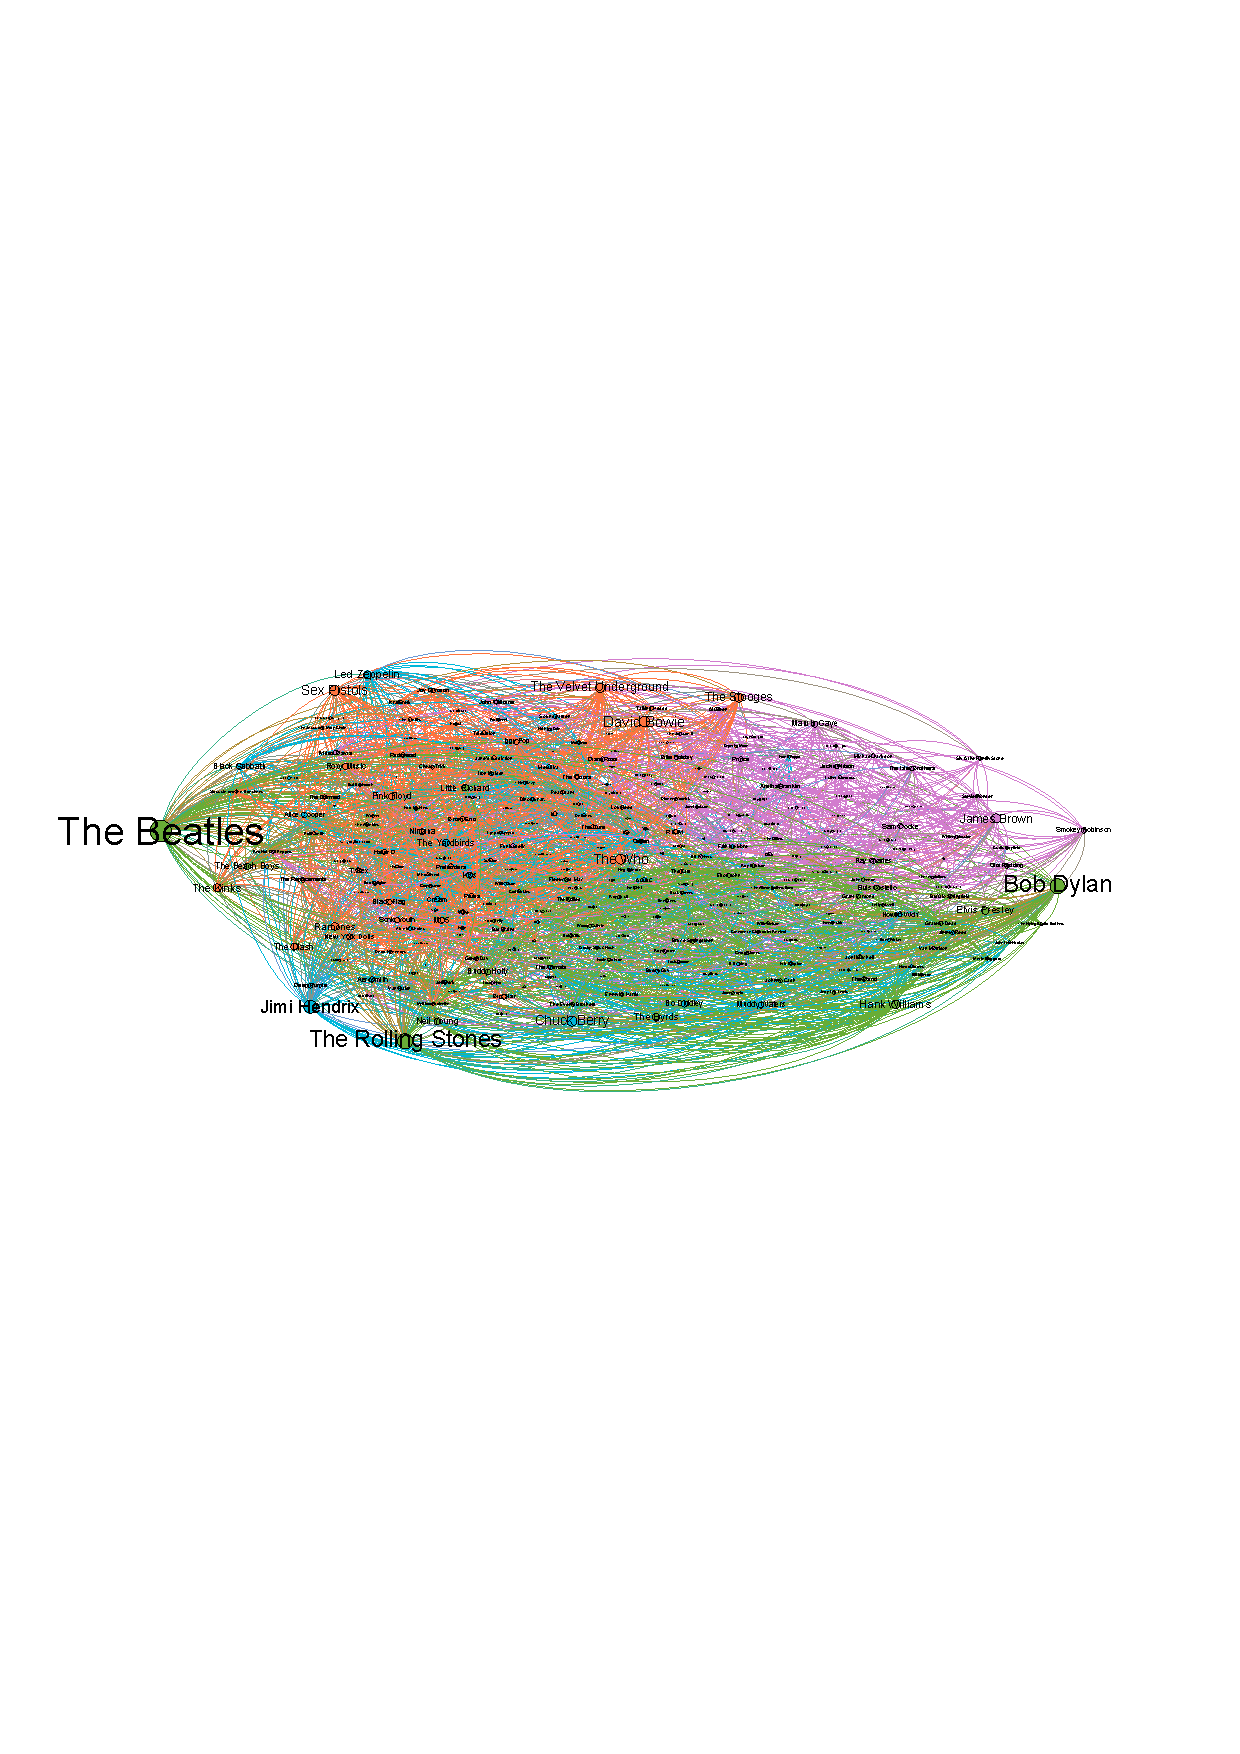
\includegraphics[width=1.1\textwidth]{Directed Influencer Network .pdf} 	% 图片相对位置
		\caption{Directed Influencer Network}		% 图片标题 
		\label{fig:in3_network}							% 图片标签
	\end{figure}
	
	
	\begin{table}[!htbp]
		\begin{center}
			\caption{Metrics of top 10 artists}
			\begin{tabular}{lllllll}
				\toprule
				\text { Id } & \text { Name } & \text { Genre } & \text { DC } & \text { WDC } & \text { EC } & \text { F-Score } \\
				\midrule
				754032 & \text { The Beatles } & \text { Pop/Rock } & 0.11 & 0.14 & 2.3 & 1.00 \\
				66915 & \text { Bob Dylan } & \text { Pop/Rock } & 0.07 & 0.1 & 1.65 & 0.68 \\
				894465 & \text { The Rolling Stones } & \text { Pop/Rock } & 0.06 & 0.07 & 1.24 & 0.52 \\
				549797 & \text { Hank Williams } & \text { Country } & 0.03 & 0.07 & 1.57 & 0.49 \\
				531986 & \text { David Bowie } & \text { Pop/Rock } & 0.04 & 0.06 & 0.71 & 0.37 \\
				354105 & \text { Jimi Hendrix } & \text { Pop/Rock } & 0.04 & 0.05 & 0.94 & 0.37 \\
				128099 & \text { James Brown } & \text { R\&B } & 0.03 & 0.05 & 1.11 & 0.36 \\
				276085 & \text { Howlin' Wolf } & \text { Blues } & 0.02 & 0.04 & 1.3 & 0.35 \\
				316834 & \text { Marvin Gaye } & \text { R\&B } & 0.03 & 0.06 & 0.72 & 0.34 \\
				139026 & \text { Led Zeppelin } & \text { Pop/Rock } & 0.04 & 0.05 & 0.65 & 0.34 \\
				\bottomrule
			\end{tabular}\label{tb:top10}
		\end{center}
	\end{table}
	
	Generally, artist with higher music influence has more followers. However, Howlin’ Wolf has less followers than Marvin Gaye, whereas has greater music influence. This is because followers of Howlin’ Wolf are more famous and influential.
	
	\section{\textsc{Task 2: } Model of Disatance between music works}
	\subsection{Data Preprocessing}
	First, we preprocess the dataset “full\_music\_data.csv”. There are 14 characteristics related
	to music included in dataset, including danceability, energy, loudness, etc. Through data visualization, we find that the Boolean variable "Explicit" is invalid: Out of 98430 tracks, only 3647 tracks are marked as 1, which means less than 4\% tracks have explicit lyrics. As it conflicts with common sense, we believe most lyrics in tracks remained undetected. Thus, we remove "Explicit" data. After that, we standardize all continuous variables
	
	Some of the music characteristics have similar meanings, for example, “energy” and “loudness” both reflect the intensity and activity of tracks. To reduce the influence of collinearity
	when calculating similarity, we use PCA (Principal Component Analysis) to reduce the dimension of the data while preserving as much of the data’s variation as possible. After calculation,
	the cumulative variance contribution rate is shown in \textbf{Table \ref{tb:CVCE}}.
	
	\begin{table}[!htbp]\footnotesize
		\begin{center}
			\caption{Cumulative Variance Contribution Rate}
			\begin{tabular}{lllllllll}
				\toprule
				\text { Number of Principal Component } & 1 & 2 & 3 & 4 & 5 & 6 & 7 & 8 \\
				\midrule
				\text { Cumulative Variance Contribution Rate } & 0.23 & 0.37 & 0.49 & 0.59 & 0.67 & 0.74 & 0.81 & 0.85 \\
				\bottomrule
			\end{tabular}\label{tb:CVCE}
		\end{center}
	\end{table}
	
	Based on the result of PCA, we choose first seven principal component and ignore the rest. The seven new variables maintain more than 80\% information of the original data
	
	\subsection{Similarity Measure and Test}
	
	Inspired by the Euclidean distance, we define music similarity between track $ i $ and track $ j $ as follows:
	
	\begin{equation}
		\operatorname{Sim}_{i j}=\frac{1}{\sqrt{\sum_{t=1}^{m}\left(x_{i t}-x_{j t}\right)^{2}}} \quad i, j=1,2, \ldots, m
	\end{equation}
	
	Comparing to other measures like Mahalanobis distance, this simple measure doesn’t need any assumption on data and is easy to calculate. 
	
	To explore whether artists in the same genre are more similar than those in different genres, we construct Mann-Whitney hypothesis test. Comparing to traditional tests such as two-sample t-test, Mann-Whitney statistic does not require distributional assumptions for its validity. In this problem, the distributions of music similarity within and between genres are quite far away from the normality. Thus, this statistic will bring about better results.
	
	We first calculate the average music similarity within genre and between genres, which can be expressed as:
	
	\begin{equation}
		\operatorname{Sim}_{i n, i}=\frac{1}{n} \sum_{j=1}^{n} \operatorname{Sim}_{i j}
	\end{equation}
	
	\begin{equation}
		\operatorname{Sim}_{b e t, i}=\frac{1}{m} \sum_{k=1}^{m} \operatorname{Sim}_{i k}
	\end{equation}
	where j, k denote individual in the same genre and different genres with artist i, and n, m denote number of above individuals, respectively.
	
	Then we calculate Mann-Whitney statistic as:
	
	\begin{equation}
		U=\frac{1}{(n+m)^{2}} \sum_{i=1}^{n+m n+m} \sum_{j=1}^{n} I\left(\operatorname{Sim}_{i n, i}<\operatorname{Sim}_{b e t, j}\right)
	\end{equation}
	
	Based on Central Limit Theorem, the asymptotic distribution of $Z=\frac{U-\frac{1}{2} n m}{\frac{1}{12} n m(n+m+1)}$ is normal distribution[4]. Based on this, we can construct Mann-Whitney Test to find out whether artists within a genre are more similar than those between genres.
	
	\subsection{Solutions}
	
	Similarity between all artists are shown in Figure 4. Mann-Whitney statistic shows that with a probability of 62.8\% and P-Value smaller than 0.001, artists within genre are more similar than those between genres.
	\clearpage
	
	\begin{figure}[htbp]
		\centering
		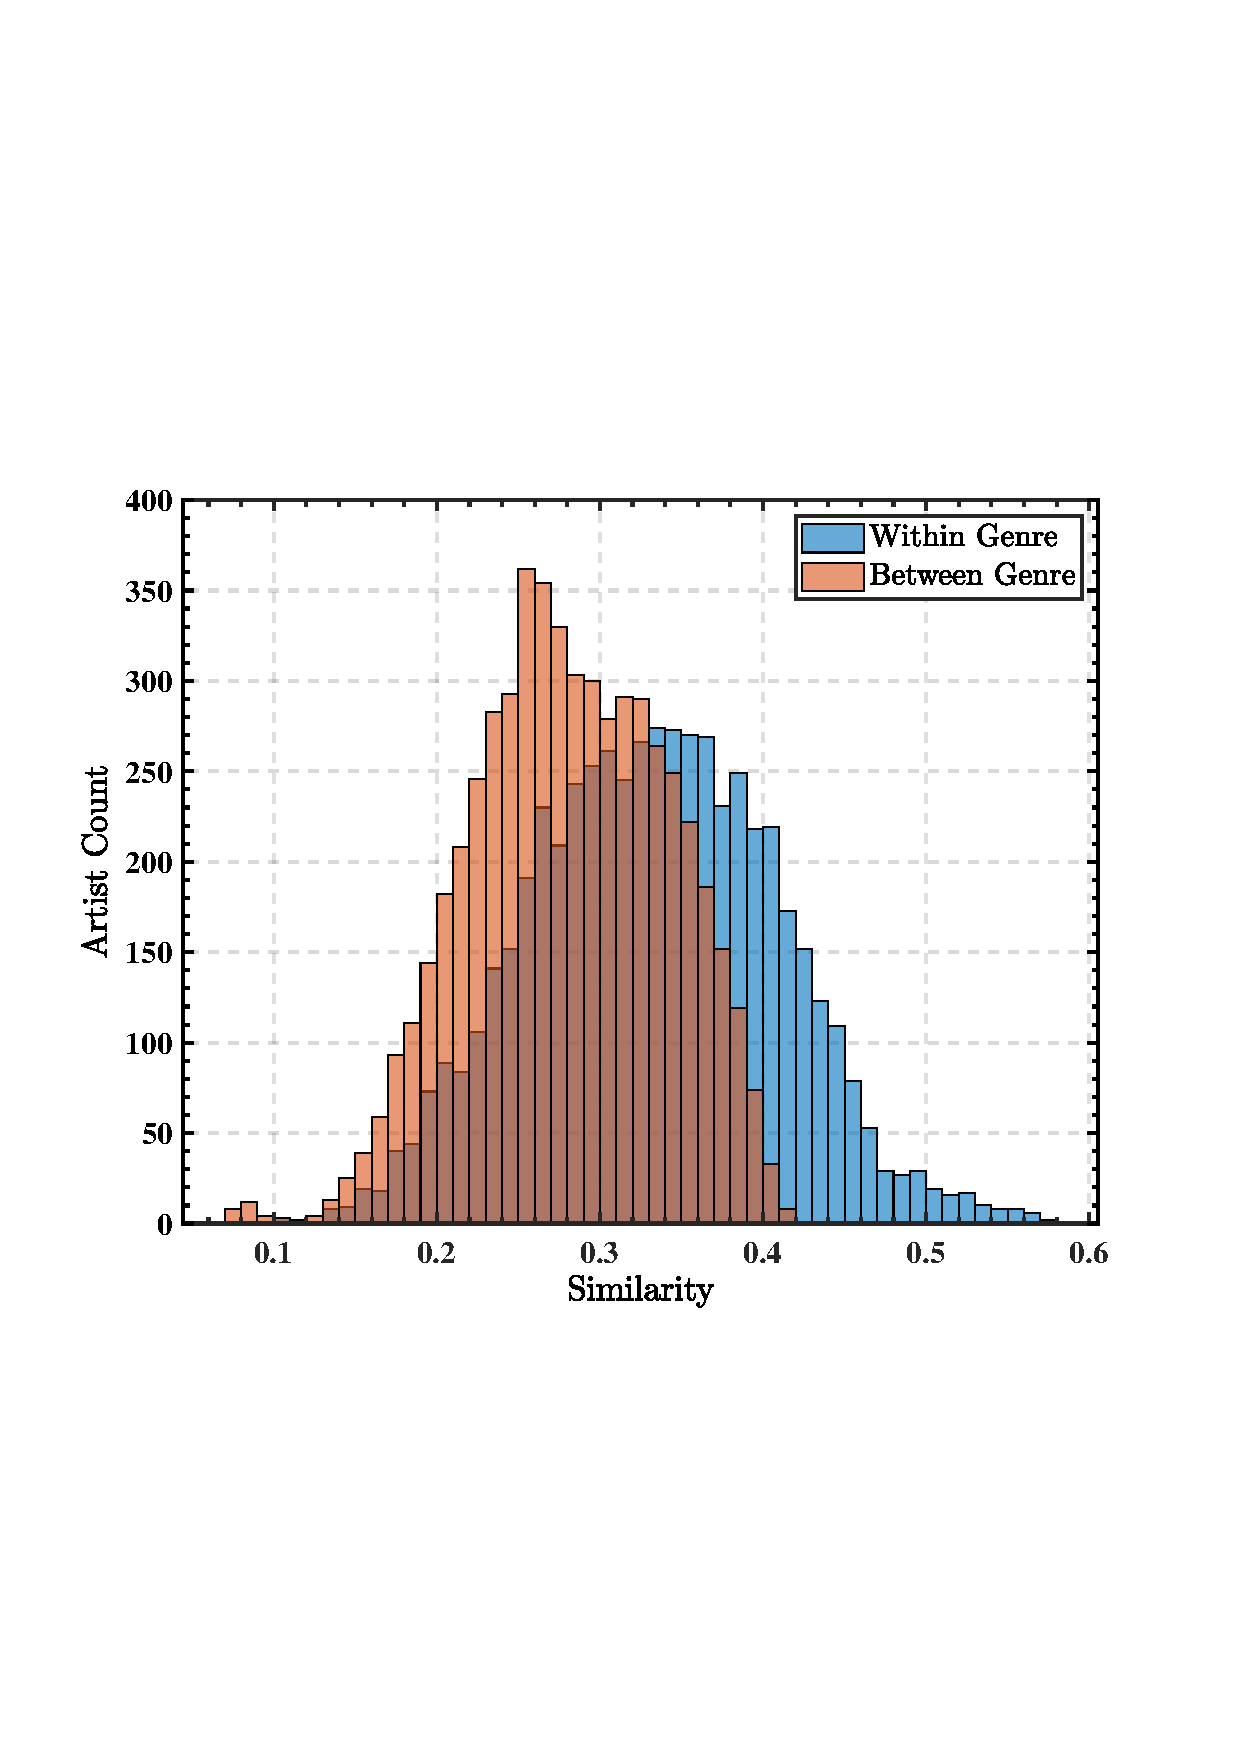
\includegraphics[width=0.7\textwidth]{sim.pdf} 	% 图片相对位置
		\caption{Similarity between artists within a genre and between genres}		% 图片标题 
		\label{fig:sim}							% 图片标签
	\end{figure}
	
	
	
	\section{\textsc{Task 3: }Build Genre Classification Tree}
	\subsection{Genre Similarity and Influence}
	
	To compare music similarity and influence on the genre level, we first merge genre in dataset "influnce\_data.csv" to dataset “data\_by\_artist.csv”, then we group the data by different genres.
	
	We define the similarity between genres as:
	
	\begin{equation}
		\operatorname{Sim}_{i j}=\frac{1}{\sqrt{\sum_{k=1}^{n_{g}}\left(c_{i k}-c_{j k}\right)^{2}}} \quad i, j=1,2, \ldots, n_{g}
	\end{equation}
	
	where $ n_g $ is the number of genres, $ c-{ik} $ is the kth average music characteristic value in genre $ i $.
	
	To evaluate the similarity within genres, we calculate the Absolute Coefficient of Variation
	of each music character in different genres, which quantifies the variation of some characteristics within genres. Let Acvi j denote the Absolute Coefficient of Variation of music character j
	in genre i, then:
	
	\begin{equation}
		A c v_{i j}=\frac{\sqrt{\frac{1}{\# G(i)} \sum_{k \in G(i)}\left(x_{j k}-\frac{1}{\# G(i)} \sum_{k \in G(i)} x_{j k}\right)^{2}}}{\left|\frac{1}{\# G(i)} \sum_{k \in G(i)} x_{j k}\right|}
	\end{equation}
	
	where $ x_{jk} $ denotes the music character $ j $ of the artist $ k $. By averaging the Acv of all continues music characters, we obtain the Average Absolute Coefficient of Variation for each genre.
	
	\subsection{Genre Classification Tree}
	
	According to our assumption, when we distinguish one genre from another, the main difference lies in the creation styles - the various features of the music created by the artists.
	Considering each genre has its unique style, we separately analyze the distinguishing features
	of each genre.
	Classification tree can distinguish the relative importance of features: A feature closer to the
	root node is more important than those closer to the leave node. The specific steps to construct
	a Genre Classfication Tree are listed as follows:
	
	\begin{enumerate}[\bfseries 1.]
		\setlength{\parsep}{2ex} %段落间距
		\setlength{\topsep}{2ex} %列表到上下文的垂直距离
		\setlength{\itemsep}{1ex} %条目间距
		\item Identify the genre to be analyzed. Mark the artists in the genre as positive and the remaining artists as negative.
		\item Construct the classification tree and choose the appropriate tree size to keep the simplicity of the classification standard.
		\item Sort the importance of features according to their relative position in the tree, visualize the tree and offer distinguishing strategy to identify the genre from others.
		
	\end{enumerate}
	
	\subsection{Solutions}
	
	\textbf{Figure \ref{fig:simm}} shows the Similarity Matrix and Influence Matrix between Genres. Blues and Easy Listening share some similar characteristics in musical features, whereas Electronic and Vocal are more similar. As for influence, Pop/Rock significantly influences other genres. Interestingly, Pop/Rock has a strong influence on R\&B, but they do not share significant similarity in musical characteristics, which we will discuss the reason later
	
	\begin{figure}[htbp]
		\centering
		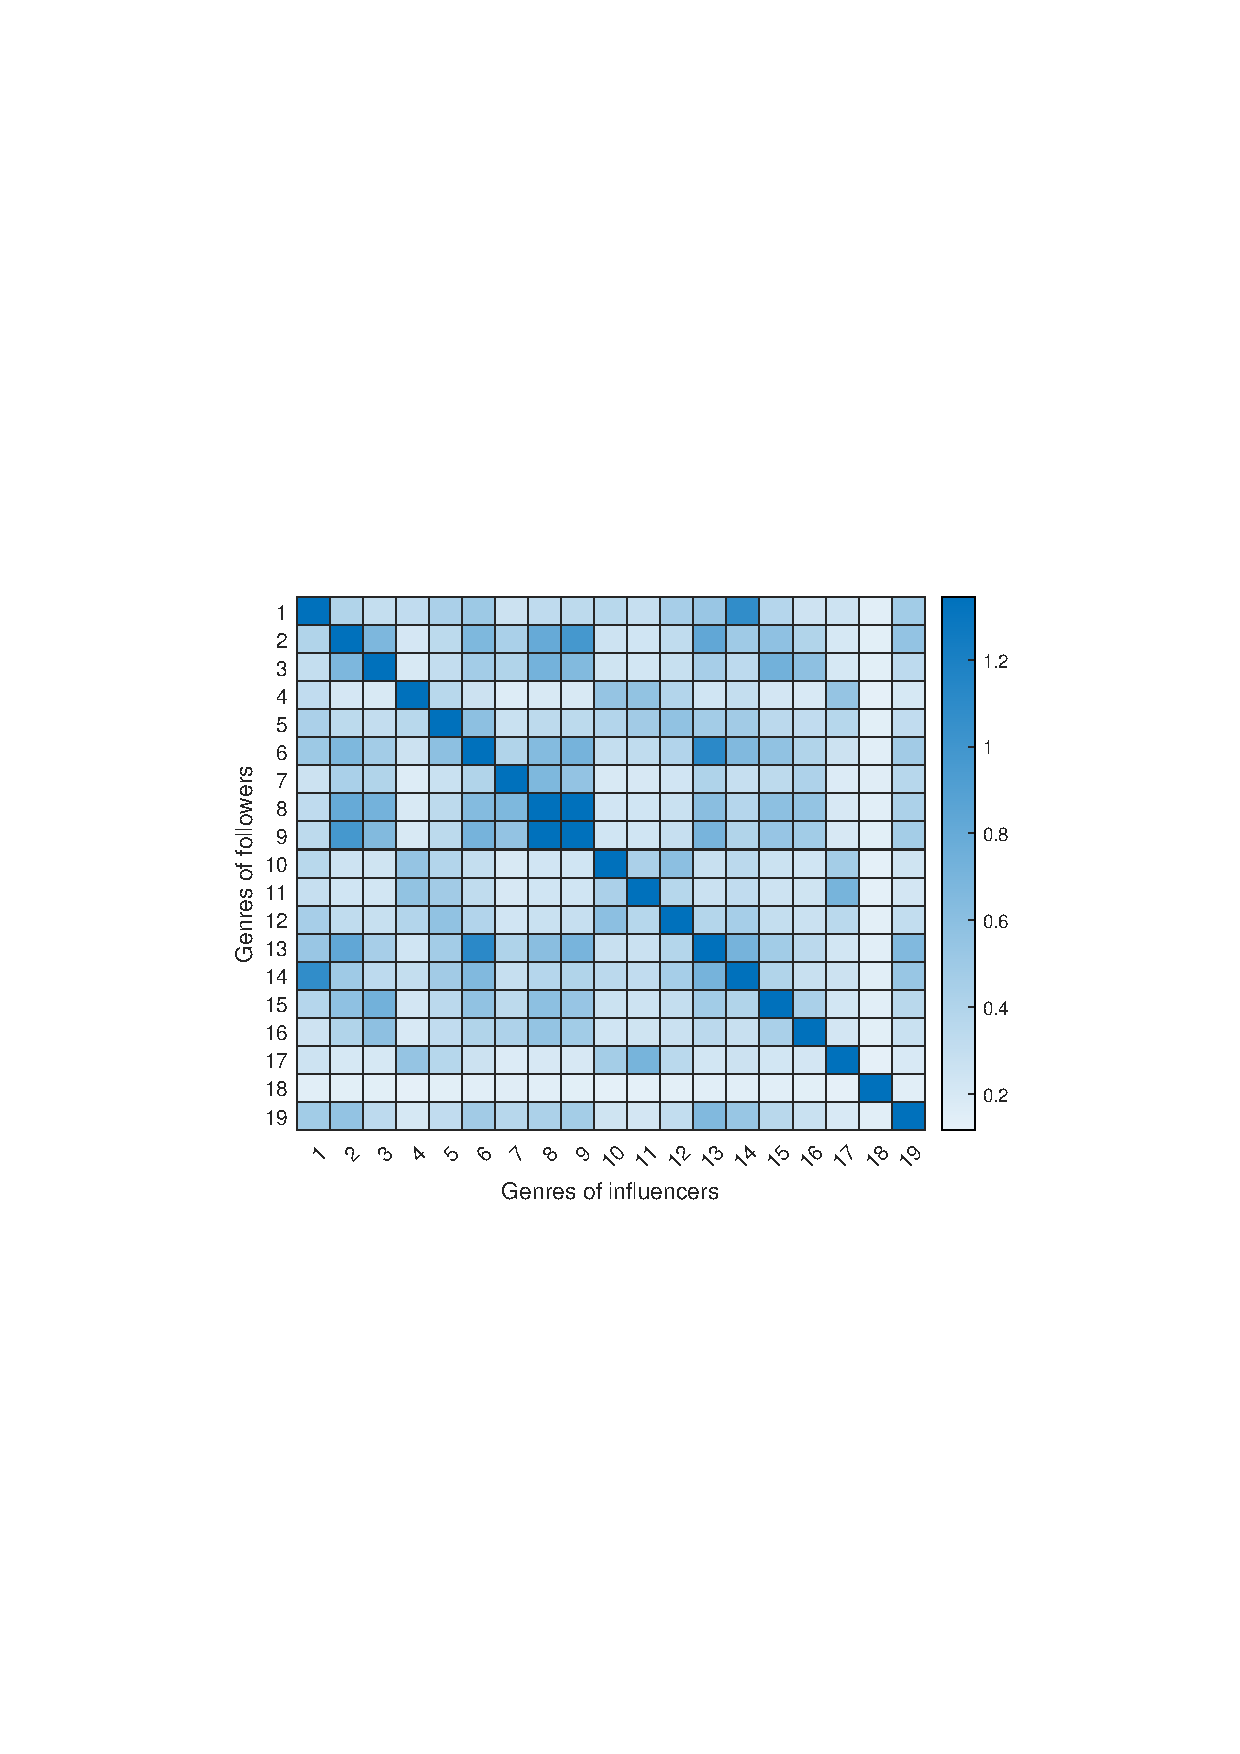
\includegraphics[width=.8\textwidth]{simm.pdf} 	% 图片相对位置
		\caption{Influence and Similarity between and within genres}		% 图片标题 
		\label{fig:simm}							% 图片标签
	\end{figure}
	
	\textbf{Figure \ref{fig:simm}} and \textbf{Figure \ref{fig:simin}} show the similarity and influence within a genre. Some genres like R\&B and Country have more variation within the genre than others, which indicates artist’s desire for true freedom of expression.At the same time, Pop/Rock and Jazz have a greater influence on themselves than others, which means they tend to maintain a consistent style.
	
	\begin{figure}[htbp]
		\centering
		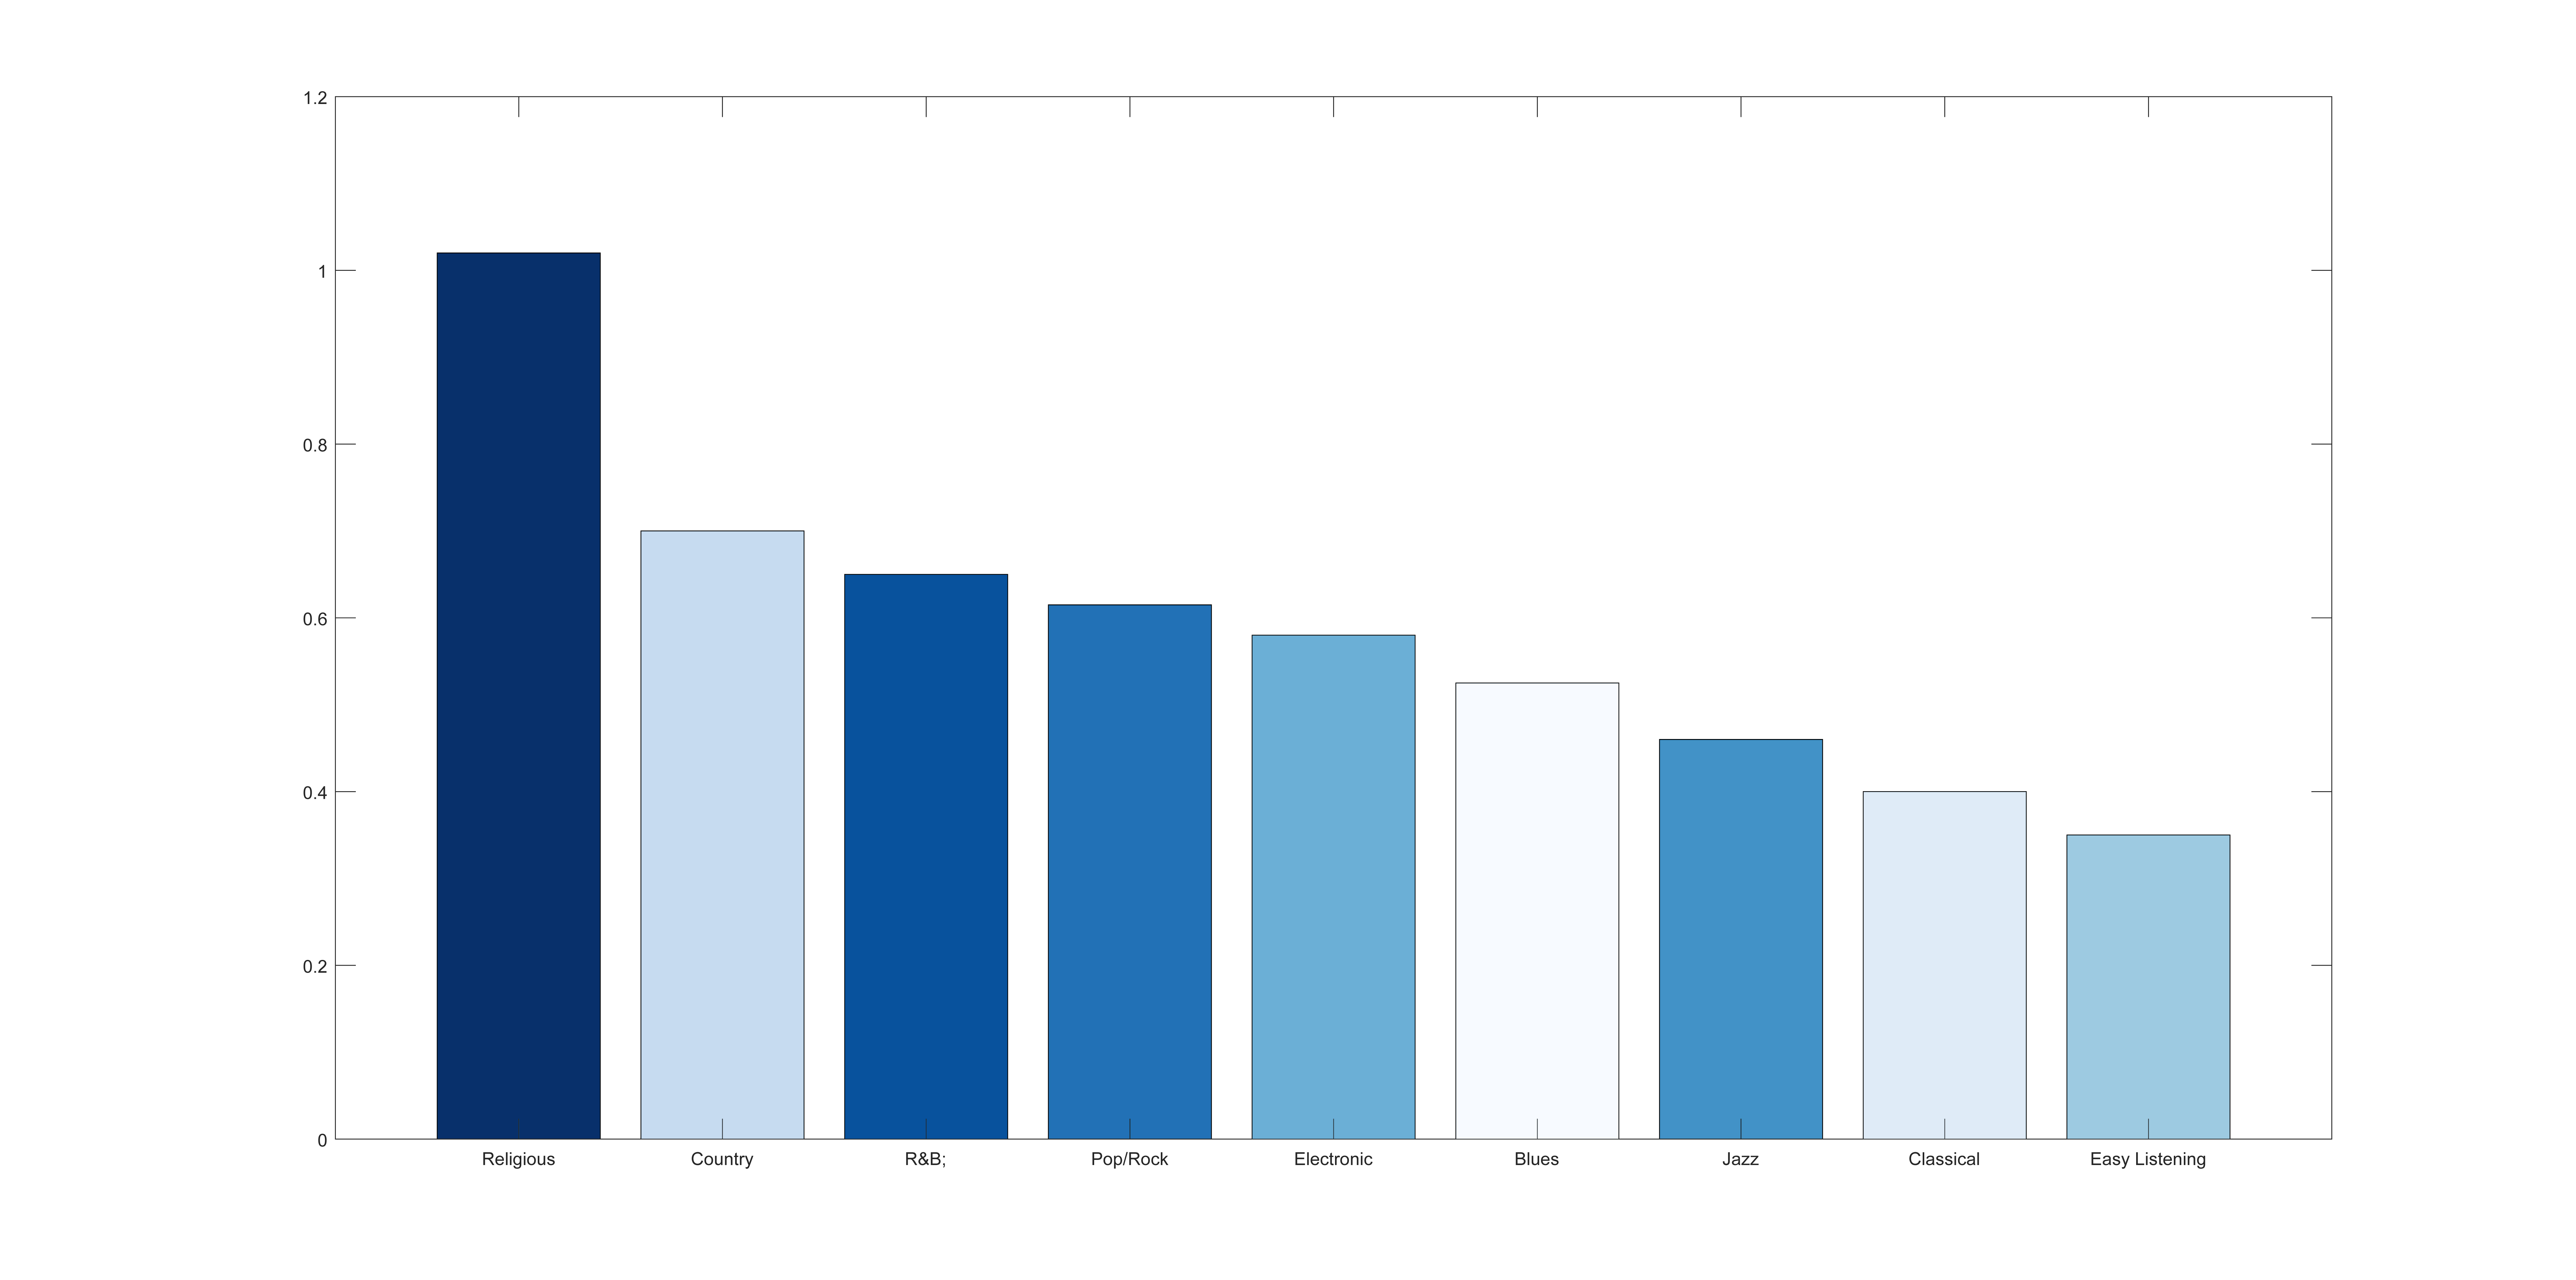
\includegraphics[width=.8\textwidth]{simin.jpg} 	% 图片相对位置
		\caption{Similarity within genres}		% 图片标题 
		\label{fig:simin}							% 图片标签
	\end{figure}
	
	\section{\textsc{Task 4}: Model of "contagious" musician}
	
	The influence\_data dataset and the data\_by\_artist dataset were used to verify whether the identified influencers actually influenced the respective artists.
	
	We stil define $ Sim_{ij} $ as:
	
	\begin{equation}\label{simij}
		\operatorname{Sim}_{i j}=\frac{1}{\sqrt{\sum_{t=1}^{m}\left(x_{i t}-x_{j t}\right)^{2}}} \quad i, j=1,2, \ldots, m
	\end{equation}
	
	where $ x_{ik} $ denotes the value of the $ k $th feature of influencer $ i $, $ x_{jk} $denotes the value of the $ k $th feature of influencer $ j $, and $ m $ denotes the total number of features referenced, $ n_p $denotes the number of influencers and influenced that appear in pairs, and the results are recorded.
	
	Then we get a ranking of similarity
	
	%TODO:a table
	
	We next explore whether it is the case that certain musical features are more "contagious" than others. We randomly selected two, three, and four features from the key features of music to form different combinations of features to recalculate the similarity of certain specific features between the influencer and the influenced. A total of $ N=C_12^2+C_12^3+C_12^4=781 $ feature combinations were used, and the data in these combinations were normalized, followed by calculations to compare whether certain specific features were more similar between influencers and influenced.
	
	\begin{equation}
		\begin{aligned}
			& \operatorname{Esim}_{\mathrm{t}}^{(\mathrm{m})}=\sum_{\mathrm{i}=1}^{\mathrm{n}_{\mathrm{p}}} \frac{1}{\mathrm{n}_{\mathrm{p}} \sqrt{\frac{\sum_{\mathrm{k}=1}^{\mathrm{m}}\left(\mathrm{x}_{\mathrm{ik}}-\mathrm{x}_{\mathrm{jk}}\right)^{2}}{\mathrm{~m}}}} 
			\mathrm{~~~~i}=\mathrm{j}=1,2, \ldots \ldots, \mathrm{n}_{\mathrm{p}} \\
			&\mathrm{m}=2 \quad \mathrm{t}=1,2, \ldots \ldots, \mathrm{C}_{12}^{2} \\
			&\mathrm{m}=3 \quad \mathrm{t}=\mathrm{C}_{12}^{2}+1, \mathrm{C}_{12}^{2}+2, \ldots \ldots, \mathrm{C}_{12}^{2}+\mathrm{C}_{12}^{3} \\
			&\mathrm{m}=4 \quad \mathrm{t}==\mathrm{C}_{12}^{2}+\mathrm{C}_{12}^{3}+1, \mathrm{C}_{12}^{2}+\mathrm{C}_{12}^{3}+2, \ldots \ldots, \mathrm{N}
		\end{aligned}
	\end{equation}
	
	where $ x_{ik} $denotes the value of the $ k $th feature of influencer $ i $, $ x_{jk} $denotes the value of the $ k $th feature of influencer $ j $, $ m $ denotes the number of features inside the referenced feature combination, $ n_p $denotes the number of influencers and influenced that appear in pairs, and $\operatorname{Esim}_{\mathrm{t}}^{(\mathrm{m})}$ represents the average similarity of the $ t $th feature combination across all influencers and influenced, which is understood as the "contagiousness" of these feature combinations.
	
	We can draw conclusions from the ranking.Not all characteristics are highly infectious to specific musicians, and the most infectious characteristics will be different for different musicians. For \textbf{Soda Stereo}, the musical feature speech is the most infectious. For \textbf{Dave Matthews}, the musical features speech and instrumentalness are the most infectious.
	
	\begin{table}[!htbp]
		\begin{center}
			\caption{Contagiousness of Musical Characteristics}
			\begin{tabular}{c|c|c|c|c}
				\toprule
				\midrule[1pt]
				\multirow{2}{*}{\textbf { Soda Stereo }} & \textbf { Characteristics } & \textit { speechiness } & \textit { energy } & \textit { instrumentalness } \\
				\cline { 2 - 5 } & \textbf{DC} & $ 0.000249 $ & $ 0.0068 $ & $ 0.007554 $ \\
				\hline \hline \multirow{2}{*}{\textbf { Dave Matthews }} & \textbf { Characteristic } & \textit { speechiness } & \textit { instrumentalness } & \textit { danceability } \\
				\cline { 2 - 5 } & \textbf{DC} & $ 8.5279 \times 10^{-5} $ & $ 9.6721 \times 10^{-5} $ & $ 0.012702 $ \\
				\midrule[1pt]
				\bottomrule
			\end{tabular}\label{tb:con}
		\end{center}
	\end{table}
	
	\section{\textsc{Task 5}: Model of Music Revolution}
	\subsection{Definition of Revolution}
	
	To tackle \textsc{Task 5}, we first define “music revolution”. The number of influencers in major
	genres is shown in figure 11. As time went by, some genre flourished and others went out of
	favor.
	
	\begin{figure}[htbp]
		\centering
		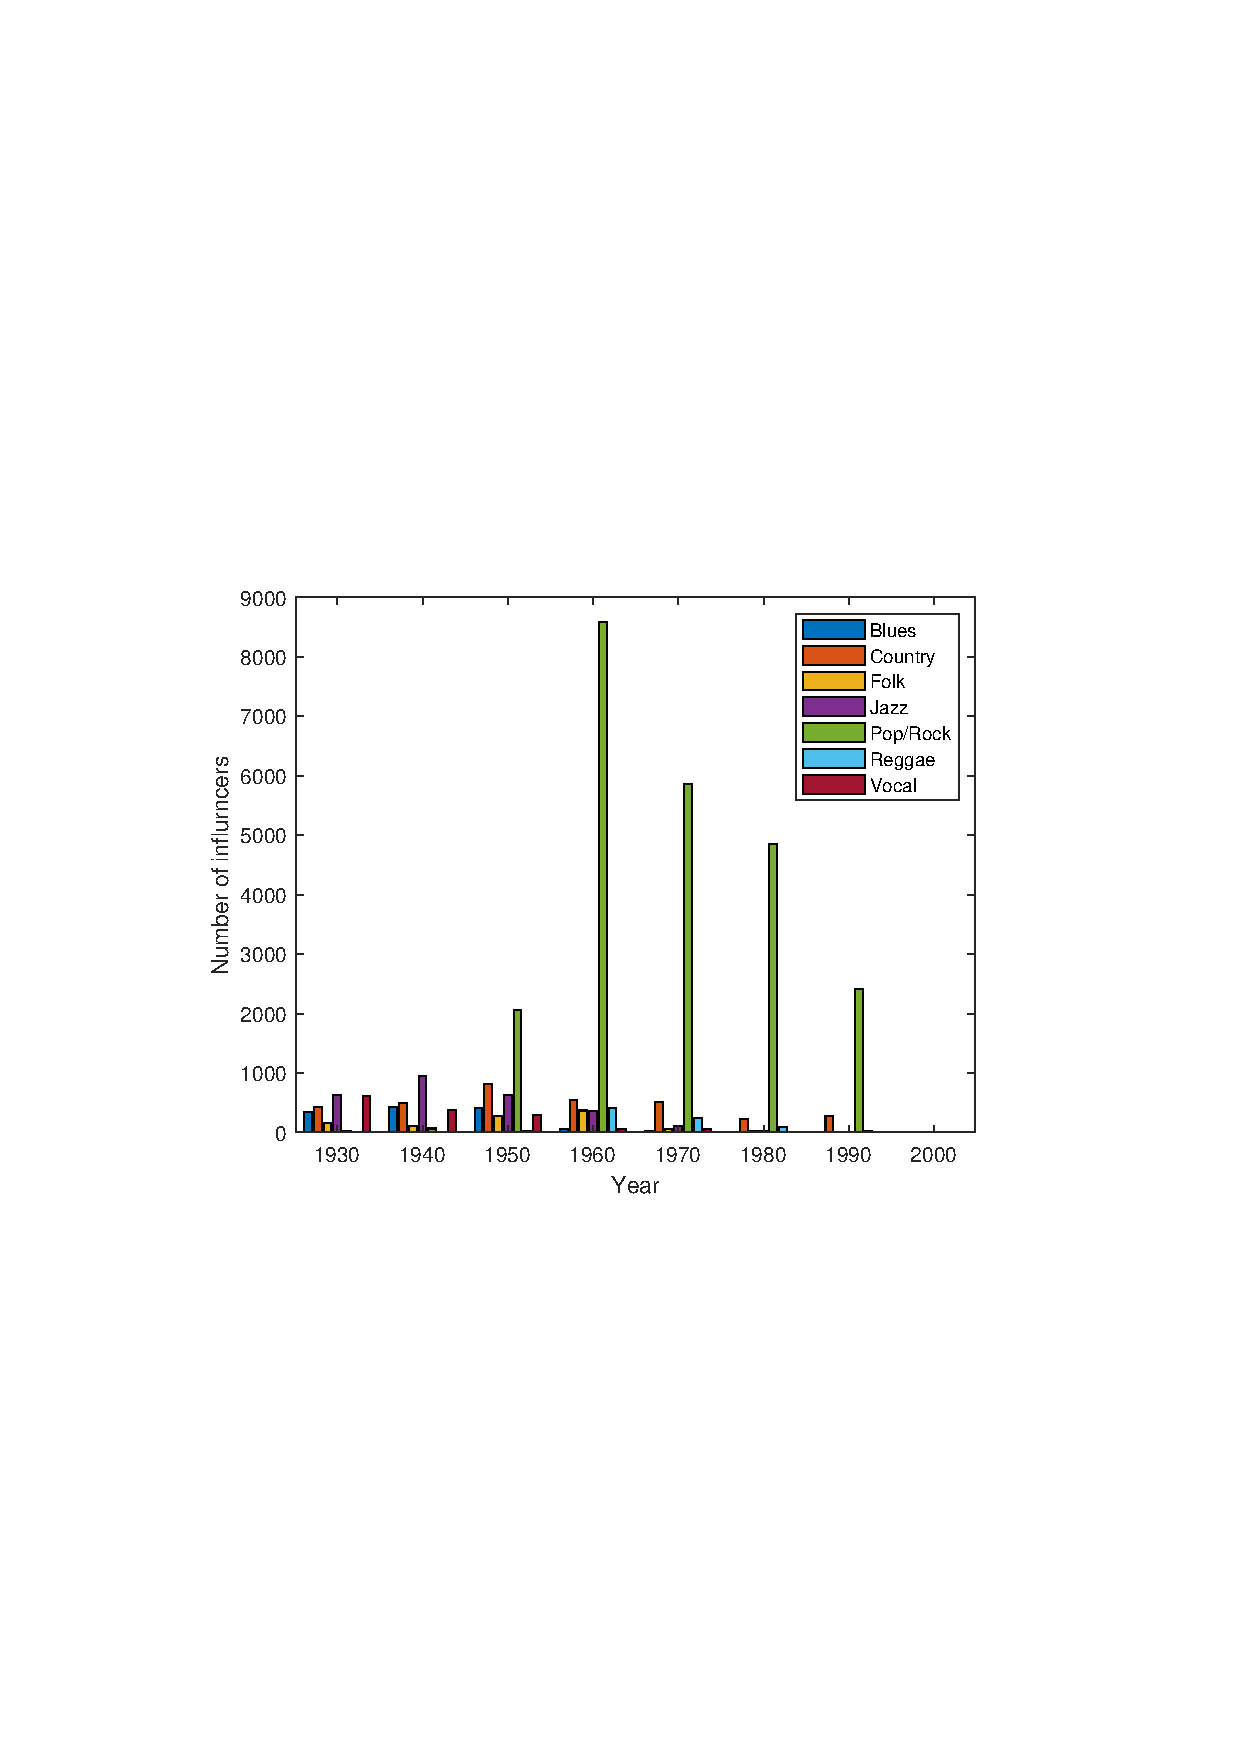
\includegraphics[width=.9\textwidth]{ig.pdf} 	% 图片相对位置
		\caption{The number of influencers in major genres}		% 图片标题 
		\label{fig:ig}							% 图片标签
	\end{figure}
	
	We define the revolution time for genres as the time when there are some genres declined and
	others springing up or dominating. From Figure 11, we find in the 1950s, Electronic flourished
	gradually, while Vocal all went from boom to bust. The popularity of Pop/Rock and R\&B also
	met a sharp increase. These phenomena indicate that 1950s is one of the revolution periods.
	
	After defining revolution periods, we focus on finding a significant change point of music
	characteristics in the 1950s to explain what we discussed above. The key to this problem is
	turned to identify the change points in time series of the music features. Based on the change
	points we find, we then can identify artists that represent the revolutionaries.
	
	\subsection{Change Points Detection (DP Algorithm)}
	
	We define the set of the change points as $ \Theta = {\{{\theta}_i\}}_{i=1}^m $. Let the time series of some music character $ {\{Y_t\}_{t=1}^n} $ admit:
	
	\begin{equation}
		Y_{t}=a_{i}+b_{i}\times\left(\frac{t}{n}\right)+\varepsilon_{t} \quad \theta_{i-1}+1 \leqslant \mathrm{t} \leqslant \theta_{i}
	\end{equation}
	where $ a_i $ is the intercept term, $ b_i $measures the speed of linear trend, and the error term $ \theta_{t} $is a white noise process.
	
	In order to ensure that the stability of parameters and change points, we also need to:
	
	\begin{equation}
		\theta_{i}-\theta_{i-1}>\tau
	\end{equation}
	and we suggest $ \tau = [0.1n] $, which will be disucssed in detail in sensitivity analysis.
	
	Since $y_{t}$ changes with a linear trend in different stages, when $\varepsilon_{i}$ follows independent and identical distribution, it is apparent to estimate parameters by minimizing the sum of squared residuals.
	
	\begin{equation}
		\left\{\theta_{i}\right\}_{i=1}^{m}=\underset{\theta \in \Theta}{\operatorname{argmin}} \sum_{t=0}^{n}\left(y_{t}-\widehat{y}_{t}\right)^{2}
	\end{equation}
	
	When the number of change points is given, the key of using Dynamic Programming algorithm in this problem is to establish the recursive relationship of the sum of squared residuals before and after a new change point is added.
	
	Let $ \delta(m, n) $ denote the sum of squared residuals associated with the optimal partition containing m breaks using first n observations, $ RSS(i, j) $ denote the sum of squared residuals obtained by applying least-squares to a segment start from $ i $ to $ j $.
	
	Then, we can achieve the global minimization of overall sum of squared residuals by solving recursive problem as follows:
	
	\begin{equation}
		\delta(m, n)=\min _{m \tau \leq j \leq n-\tau} \boldsymbol{\delta}(m-1, j)+\operatorname{RSS}(j+1, n)
	\end{equation}
	where $ \tau $ is a trimming parameter that constrains the distance between two change points not to be too close.
	
	It is important to note that the DP algorithm is O(T2) and does not depend on the number of change points. Therefore, we can quickly estimate all the change points which are consistent for real ones[5].
	
	Obviously, we also need to penalize the number of change points. Considering the number of change points as a tuning parameter, We recommend to use BIC criterion to determine the optimal number of change points $ m^{*} $.
	
	\begin{equation}
		m^{*}=\underset{m}{\operatorname{argmin}} R S S_{\text {overall }}+\log (n) * \widehat{\sigma}^{2} * m
	\end{equation}
	
	\subsection{Solutions}
	
	\begin{figure}[htbp]
		\centering    
		\subfigure[Energy]{				% 图片1([]内为子图标题)
			\label{p1}							% 子图1的标签
			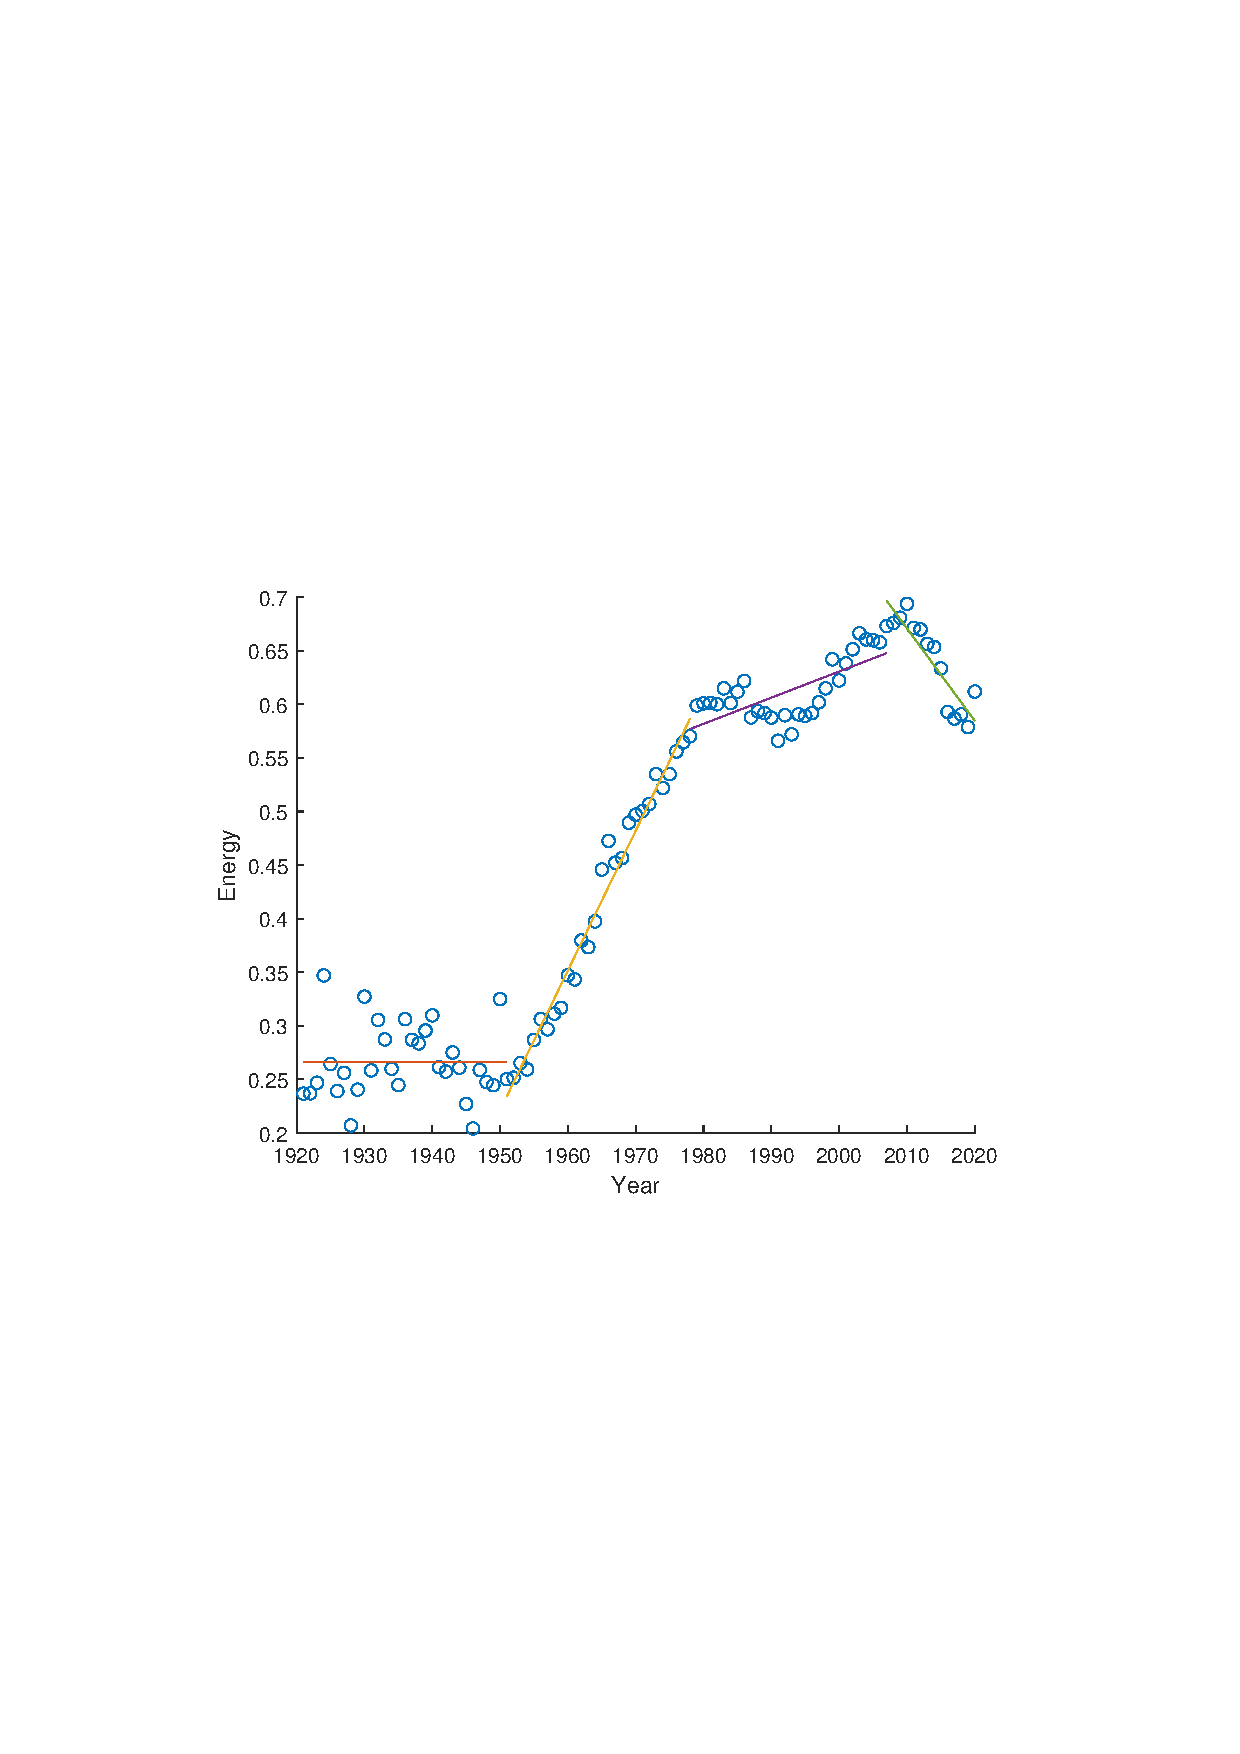
\includegraphics[width=0.45\textwidth]{p1.pdf}}			  % 子图1的相对位置
		\subfigure[Acousticness]{				% 图片2
			\label{p2}						% 子图2的标签
			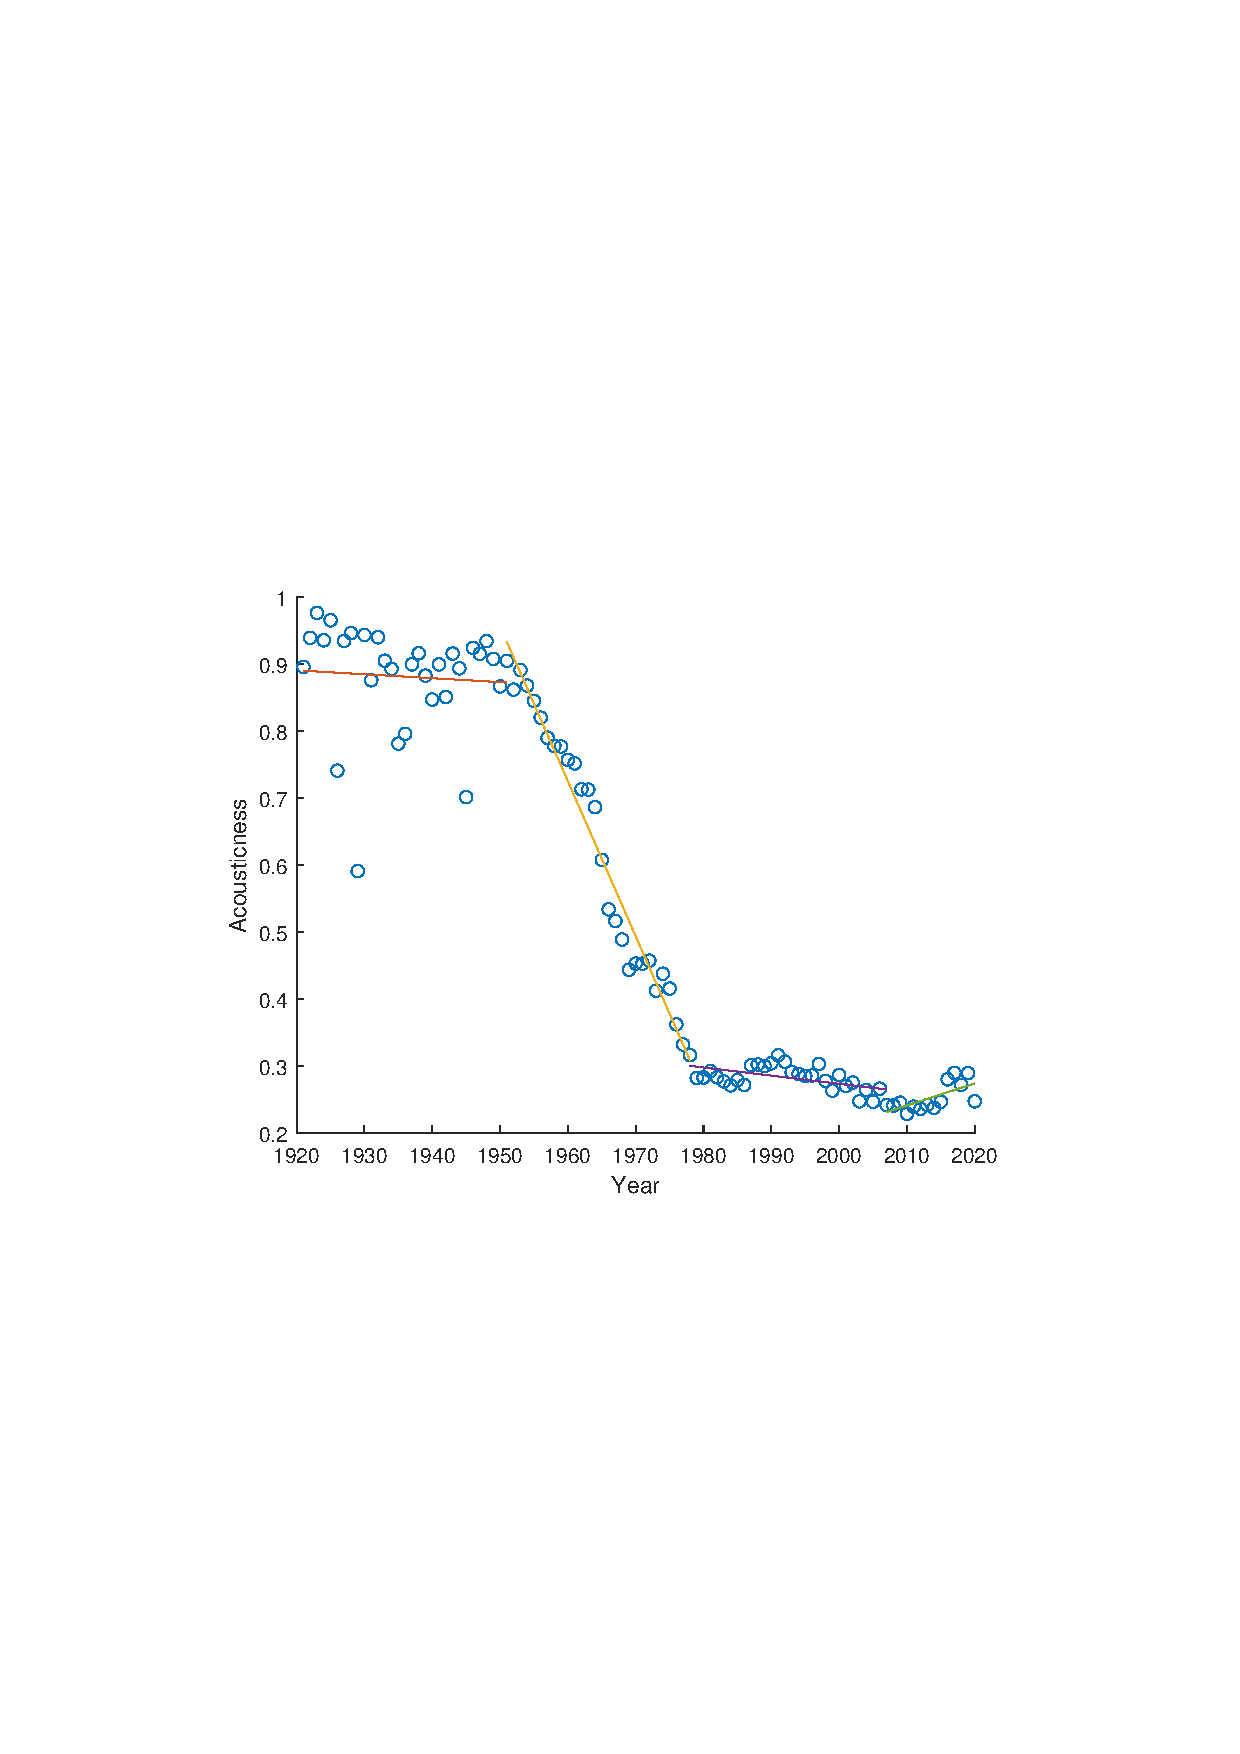
\includegraphics[width=0.45\textwidth]{p2 .pdf}}
		\caption{Change points detection of acousticness and energy}		% 总图标题
		\label{Fig:cp}									% 总图标签
	\end{figure}
	
	
	
	By using the DP algorithm above, we detected the change points of 11 continuous music
	characteristics in the dataset “data\_by\_year.csv”, as shown in \textbf{Table \ref{tb:revo}}.
	
	It can be seen in \textbf{Table \ref{tb:revo}} that four music characters (acousticness, energy, danceability and loudness) show significant changes around 1950.
	
	
	\begin{table}[!htbp]
		\begin{center}
			\caption{Revolution date of music characteristics}
			\begin{tabular}{lcccccccc}
				\toprule
				& \multicolumn{8}{c}{\text { Revolution date }} \\
				\cline { 2 - 9 } 
				\text { Characteristic } & $ 1930 \mathrm{~s} $ & $ 1940 \mathrm{~s} $ & $ 1950 \mathrm{~s} $ & $ 1960 \mathrm{~s} $ & $ 1970 \mathrm{~s} $ & $ 1980 \mathrm{~s} $ & $ 1990 \mathrm{~s} $ & $ 2000 \mathrm{~s} $ \\
				\midrule[1pt]
				\text { Instrumentalness } & 1933 & 1946 & - & 1964 & - & - & - & - \\
				\text { Duration\_ms } & - & 1946 & - & 1966 & - & - & - & 2007 \\
				\text { Acousticness } & - & - & $ \mathbf{1 9 5 0} $ & 1964 & 1979 & - & - & - \\
				\text { Tempo } & - & 1947 & - & - & 1979 & - & 1996 & 2008 \\
				\text { Danceability } & - & - & $ \mathbf{1 9 5 0} $ & - & - & - & 1997 & 2008 \\
				\text { Valence } & - & 1947 & - & 1966 & - & - & - & 2005 \\
				\text { Energy } & - & - & $ \mathbf{1 9 5 1} $ & - & 1979 & - & - & 2008 \\
				\text { Liveness } & - & - & 1956 & - & 1976 & - & - & 2008 \\
				\text { Speechness } & - & - & 1956 & - & - & - & - & 2006 \\
				\text { Popularity } & - & - & 1953 & - & 1970 & - & - & 2006 \\
				\text { Loudness } & 1936 & - & $ \mathbf{1 9 5 0} $ & - & - & - & - & 2008 \\
				
				\bottomrule
			\end{tabular}\label{tb:revo}
		\end{center}
	\end{table}
	
	To get a further insight into the revolution related to music characteristics in different genres, we draw boxplots of energy and acousticness respectively in figure 13. Obviously, the new genres (Pop/Rock, R\&B and Electronic) have significant higher energy, yet their acousticness is much lower than the old ones. This is consistent with the time series analysis above. Thus, we convinced that the four music characters: acousticness, energy, danceability and loudness might signify revolutions in musical evolution.
	
	\begin{figure}[htbp]
		\centering    
		\subfigure[Energy]{				% 图片1([]内为子图标题)
			\label{box1}							% 子图1的标签
			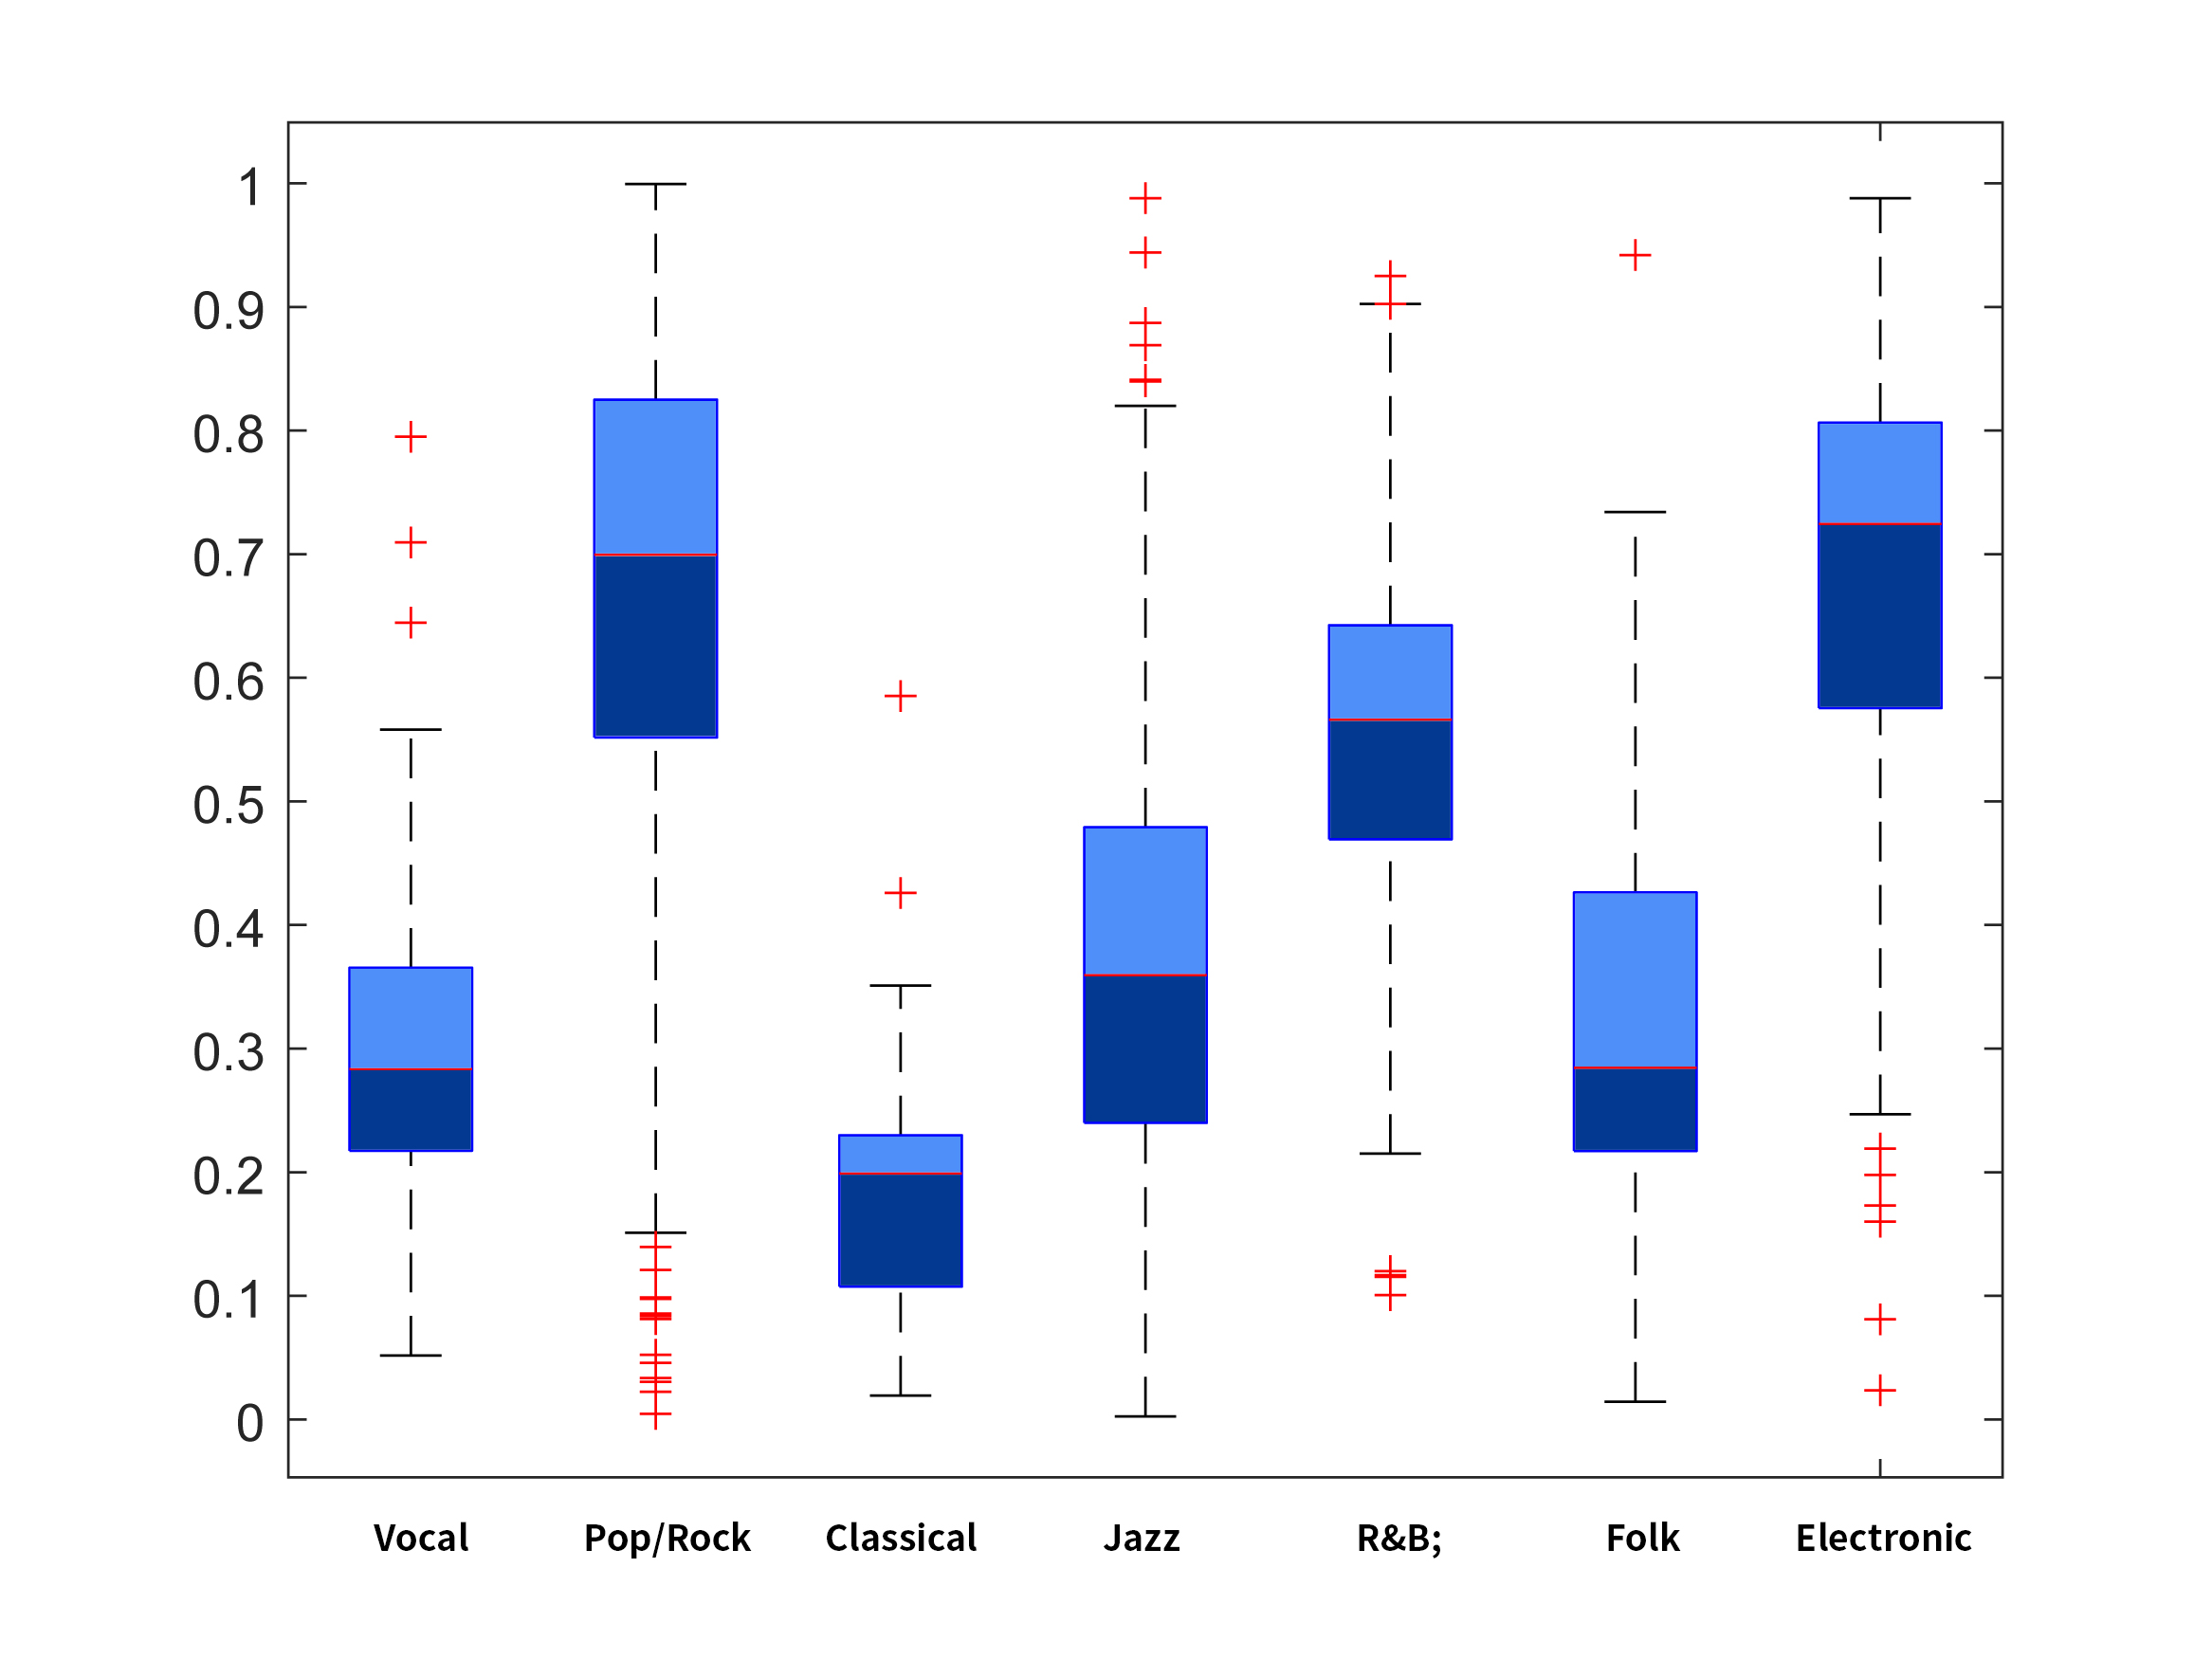
\includegraphics[width=0.4\textwidth]{box1.jpg}}			  % 子图1的相对位置
		\subfigure[Acousticness]{				% 图片2
			\label{box2}						% 子图2的标签
			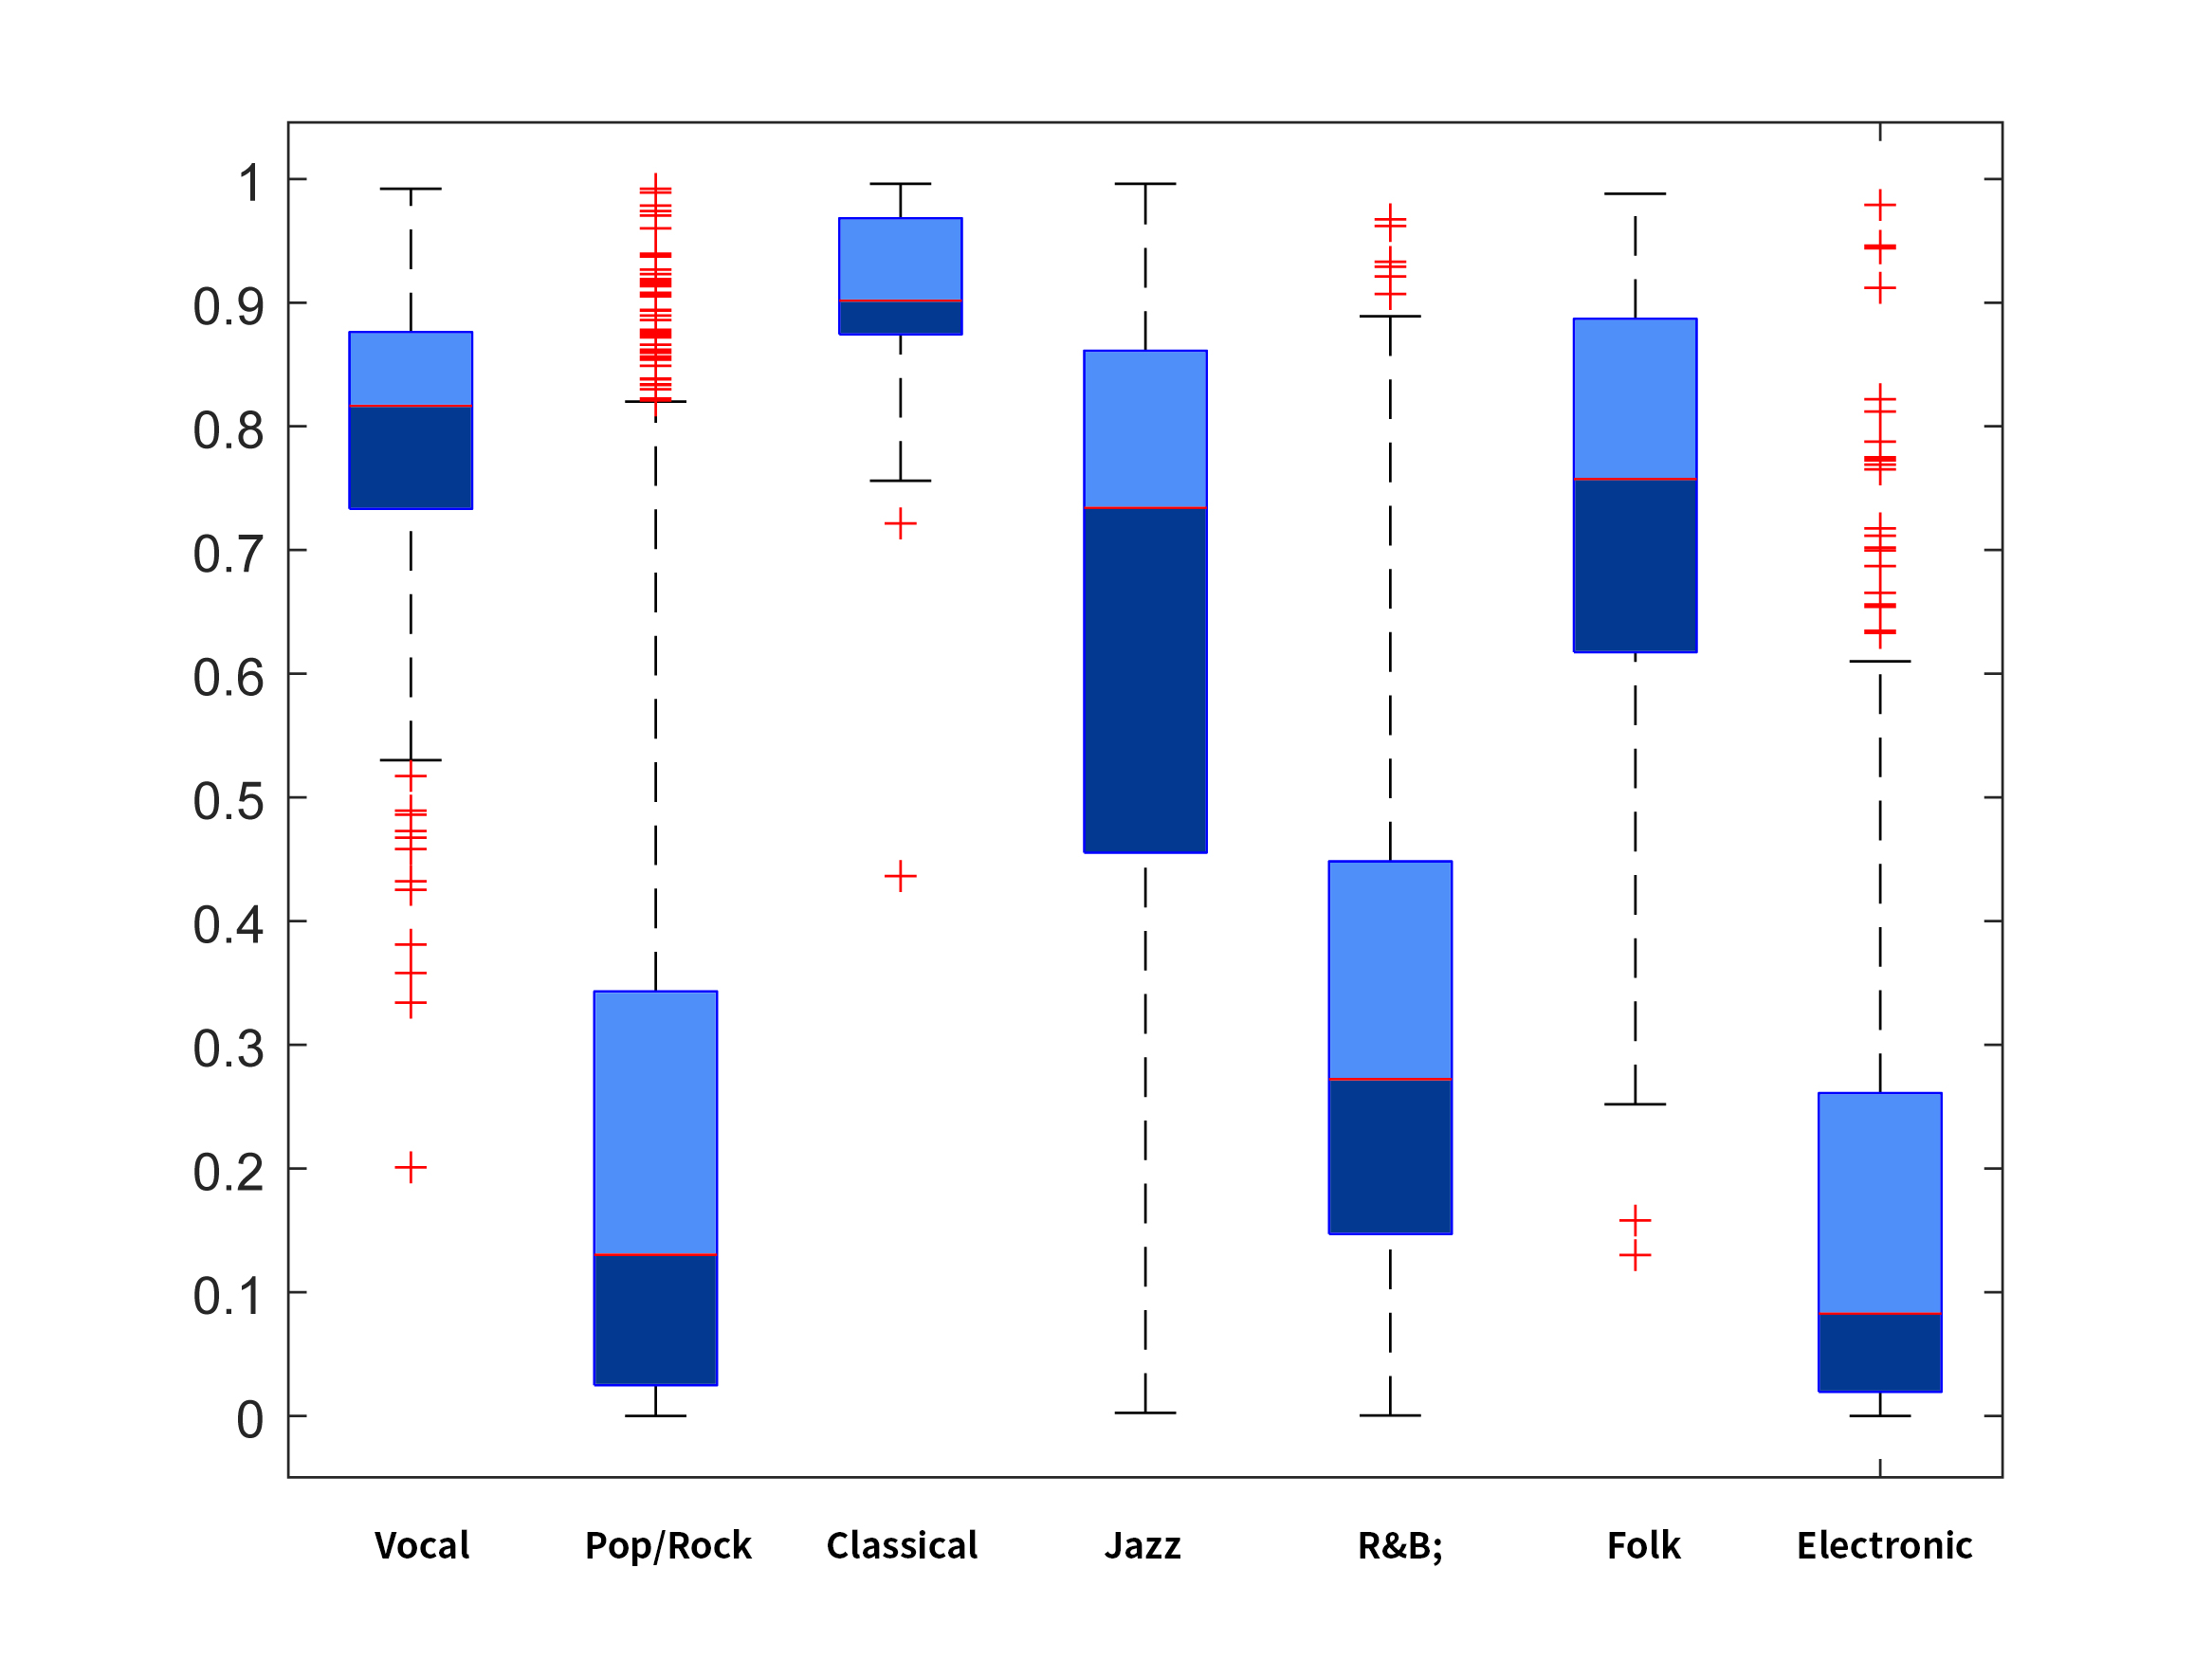
\includegraphics[width=0.4\textwidth]{box2.jpg}}
		\caption{Energy and Acousticness in different genres}		% 总图标题
		\label{Fig:box}									% 总图标签
	\end{figure}
	
	For the year corresponding to a genre change, I analyze the music published in the two years before and after the internal change of the genre, and look for the most popular artists in this period. We sum the popularity of the works published by each musician during this period, and get the popularity of each musician during this period. The highest is the main influencer in the reform. Electronic was analyzed using the above method.
	
	In 1950, freestyle's works had the highest sum of population: 144, which was the main influencer of the change in 1950. In 1969, \textbf{Jean Jacques perrey}'s works had the highest sum of popularity: 139, which was the main influencer of the change in 1969.
	
	From the beginning of the reform in 1969 to 1978, the trend of change has been maintained. We believe that a long-term change has taken place during this period. We also find out that the main influencers in the vicinity from 1969 to 1979 are \textbf{kraftwerk}: sum of population = 822, \textbf{Yellow Magic Orchestra}: sum of population = 495, Vangelis: sum of population = 473
	
	\section{\textsc{Task 6}: Model of Dynamic Influencer}
	
	\subsection{Dynamic Influencer Indicator}
	
	In this task, we choose Pop Rock as the genre for research since it exists for a long time andthere are several reinventions.
	Intuitively,dynamic influencers dramatically change the trend of the genre in a specificperiod of time. Thus a dynamic influencer of a period should satisfy
	
	\begin{enumerate}
		\setlength{\parsep}{2ex} %段落间距
		\setlength{\topsep}{2ex} %列表到上下文的垂直距离
		\setlength{\itemsep}{1ex} %条目间距
		\item He/She released more than 10 tracks in this period.
		\item The music characteristics of these tracks are consistent with the lagging trend of Pop/Rock.
	\end{enumerate}
	
	Based on the definition above, we construct an indicator of dynamic influencer as:
	
	\begin{equation}
		d_{i}=\frac{1}{\left|A_{i}\right|} \sum_{t \in A_{i}}\left(\sum_{j \in F}\left(x_{i, j, t}-\bar{x}_{j, t-v}\right)^{2}\right)^{\frac{1}{2}}
	\end{equation}
	where$  x_{i,j,t} $ is the music characteristics $ j $ of tracks released by the $ i $th artist in the year $ t $,  $\bar{x}_{j, t}$ is the average value of artists, $ F $ is the set of music characteristics, $ v $ is the lag year. Here we set $ v $ = 1 , which means the dynamic influencer will lead the music trend a year after tracks are released.
	
	\subsection{Solutions}
	
	Changes of music characteristics in Pop/Rock are shown in \textbf{Figure \ref{fig:9}} Preliminary data analysis shows that most Pop/Rock songs are released after 1956 (the dotted line). Before 1956, the fluctuation of musical characteristics is caused by small sample size. Therefore, we only analyze changes after 1956. We set 
	\begin{equation}
		F=\{\text { acousticness, danceability, energy,loudness, valence }\}
	\end{equation}
	as only these characteristics show significant fluctuations after 1956.
	\clearpage
	\begin{figure}[htbp]
		\centering
		\includegraphics[width=1\textwidth]{9.jpg} 	% 图片相对位置
		\caption{Changes of music characteristics in Pop/Rock}		% 图片标题 
		\label{fig:9}							% 图片标签
	\end{figure}
	
	By calculating the value of dynamic influencer indicator of 99 most famous artists, we find
	out top 10 dynamic influencers that have giant impact on Pop/Rock. The influencer and his/her
	active period is shown in \textbf{Figure \ref{fig:pr10}}
	
	\begin{figure}[htbp]
		\centering
		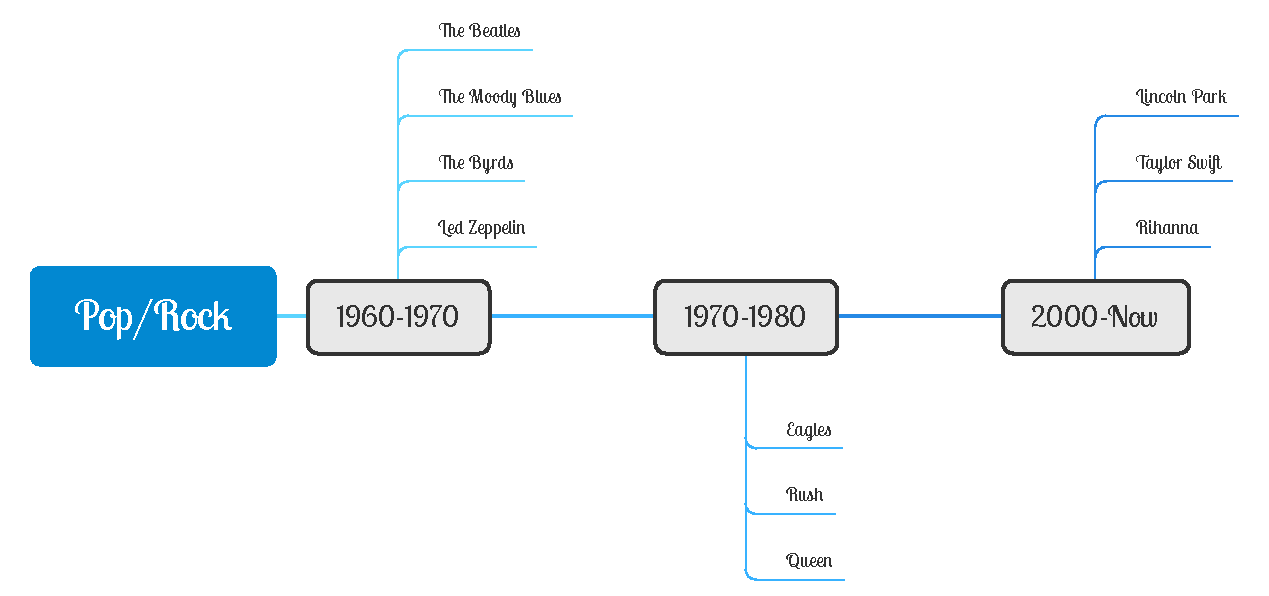
\includegraphics[width=1.1\textwidth]{pRock.pdf} 	% 图片相对位置
		\caption{Changes of dynamic influencer in Pop/Rock}		% 图片标题 
		\label{fig:pr10}							% 图片标签
	\end{figure}
	
	According to the figure 15, Some music characteristics of Pop/Rock have changed a lot over
	time. Acousticness and valence both experience a significant decline after 1956, while energy
	and loudness show a consistent increase.
	
	The change above is mainly caused by the change of dynamic influencers. With the technology enhancements and electrical amplification, the Beatles, Led Zeppelin and Eagles poured
	more intense emotion and passion into Pop Rock music in the last century. These artists tend to
	express sadness or depressed emotions. However, in recent 20 years, some great musicians, like
	Lincoln Park and Taylor Swift, switched the tone of Pop Rock music from sadness to happiness.
	They make pop music smooth, relaxing and much more suitable for dancing.
	
	\section{\textsc{Task 7}: The influence of external aspects}
	\subsection{Cultural Influence of music}\label{sec7.1}
	
	Based on the models in the previous section, we detect three important periods in musical evolution, as shown in \textbf{Figure \ref{Fig:cip}}. We discuss the culture-influence processes as follows:
	
	\begin{figure}[htbp]
		\centering    
		\subfigure[Tempo]{				% 图片1([]内为子图标题)
			\label{Fig.sub.match1}							% 子图1的标签
			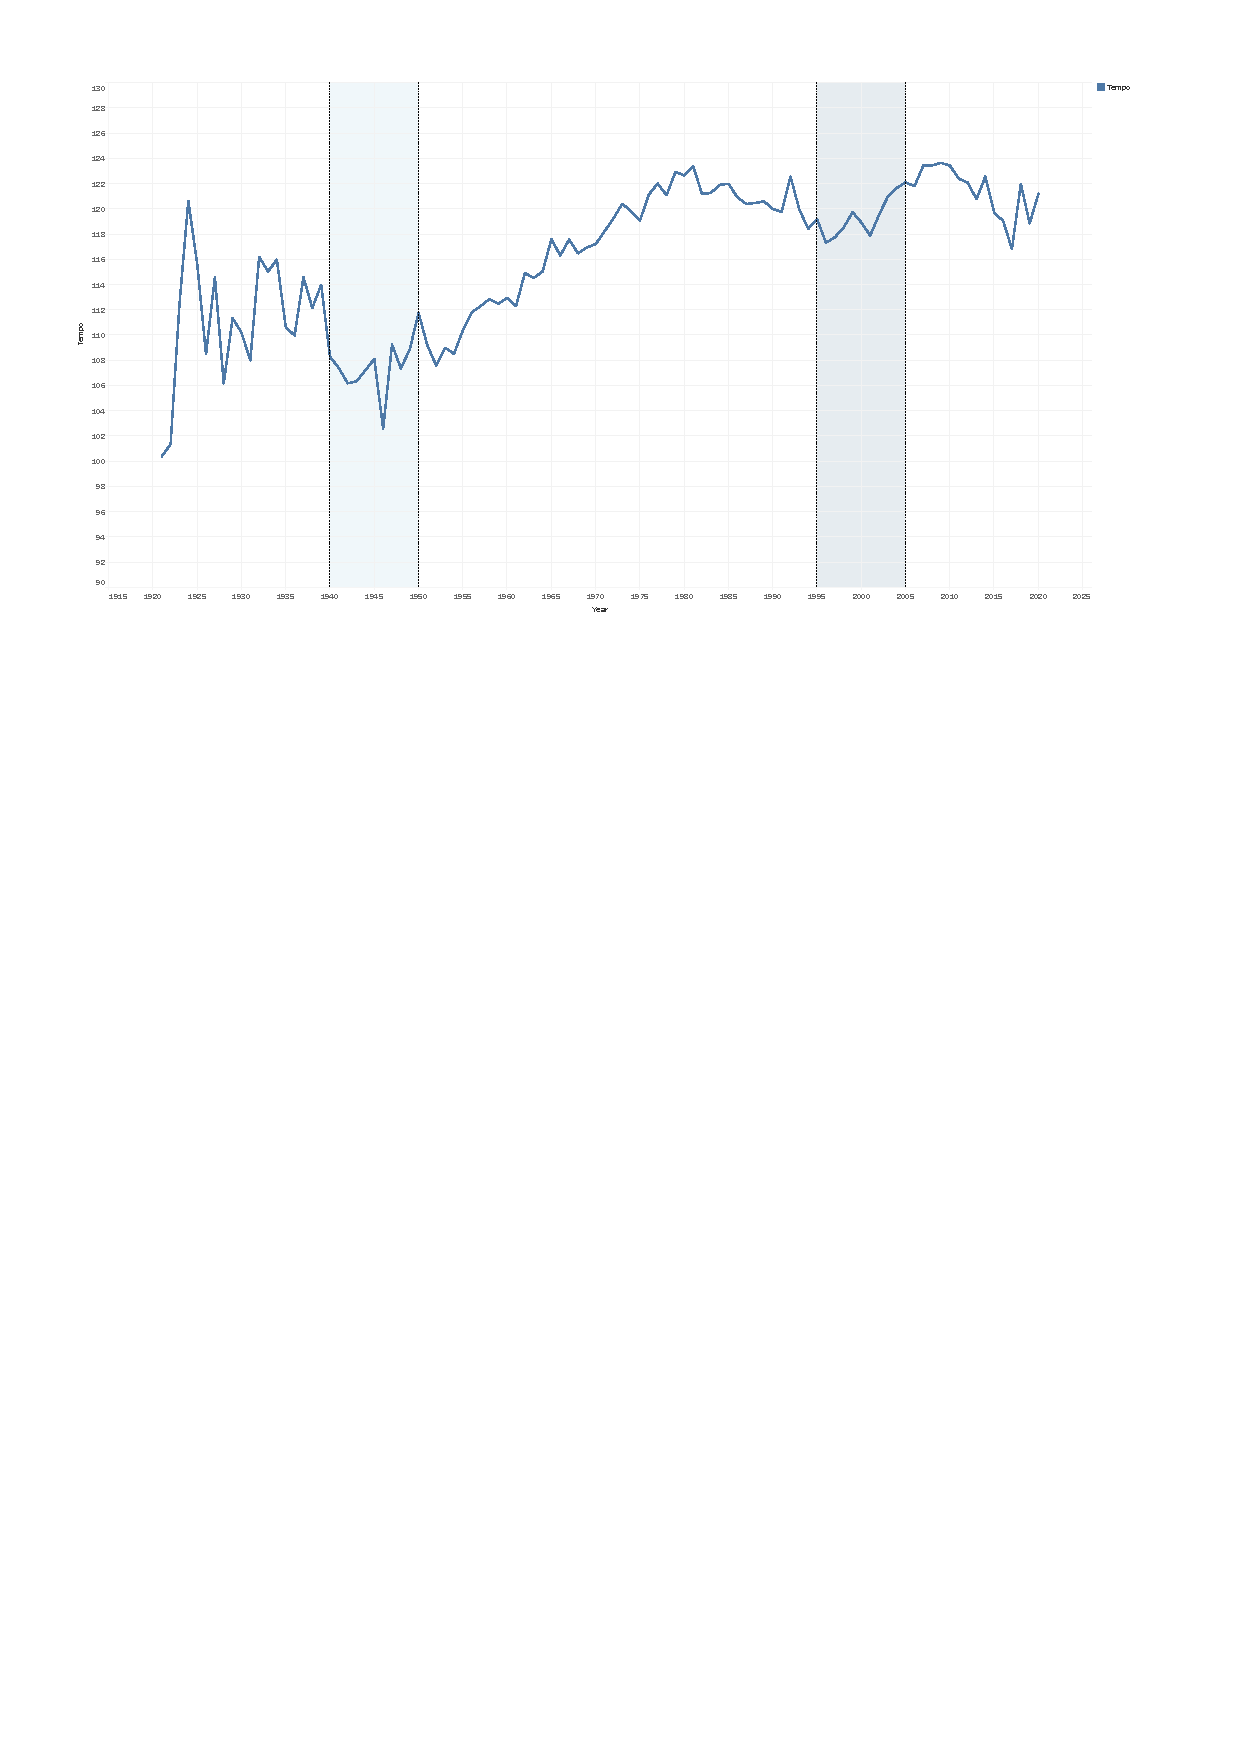
\includegraphics[width=0.4\textwidth]{qushi1.pdf}}			  % 子图1的相对位置
		\subfigure[Energy]{				% 图片2
			\label{Fig.sub.match2}						% 子图2的标签
			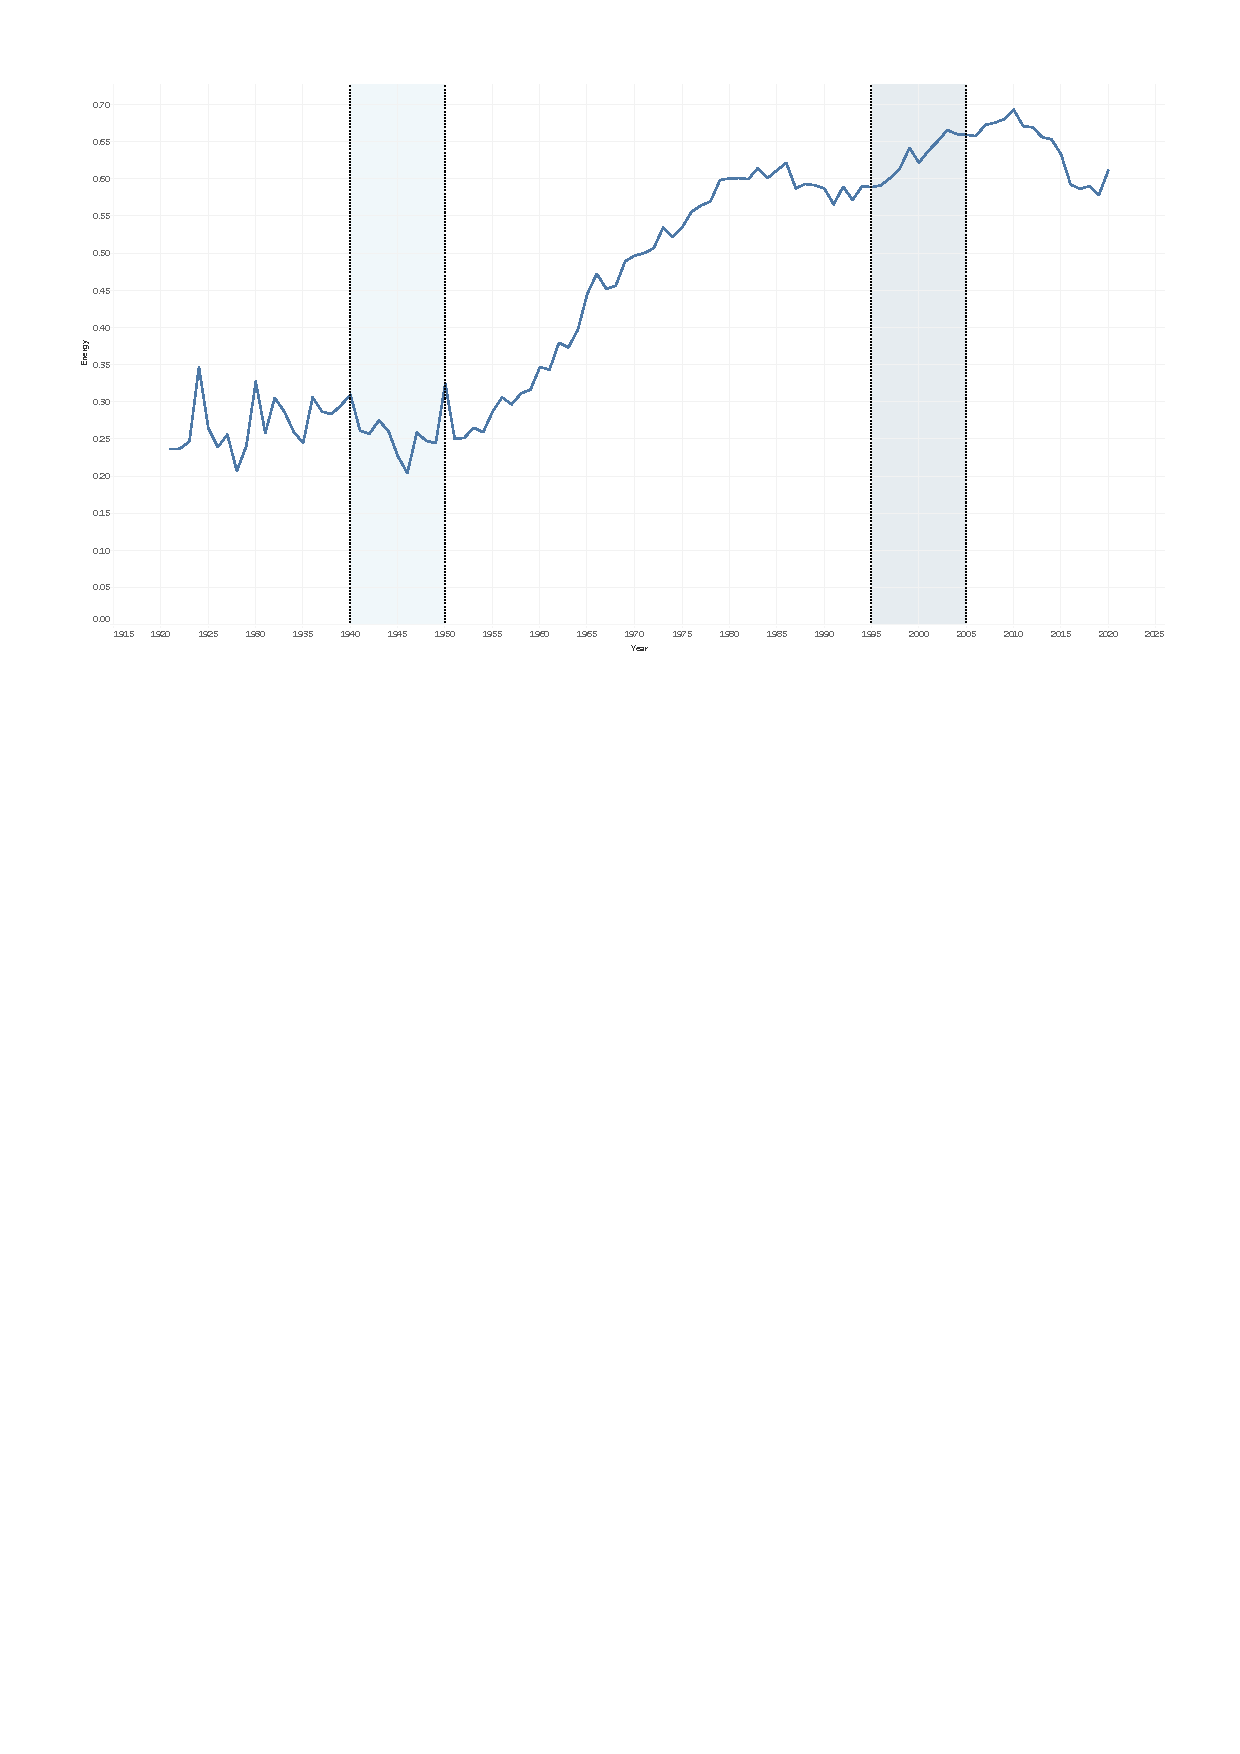
\includegraphics[width=0.4\textwidth]{qushi2.pdf}}
		\subfigure[Danceability]{				% 图片1([]内为子图标题)
			\label{Fig.sub.match3}							% 子图1的标签
			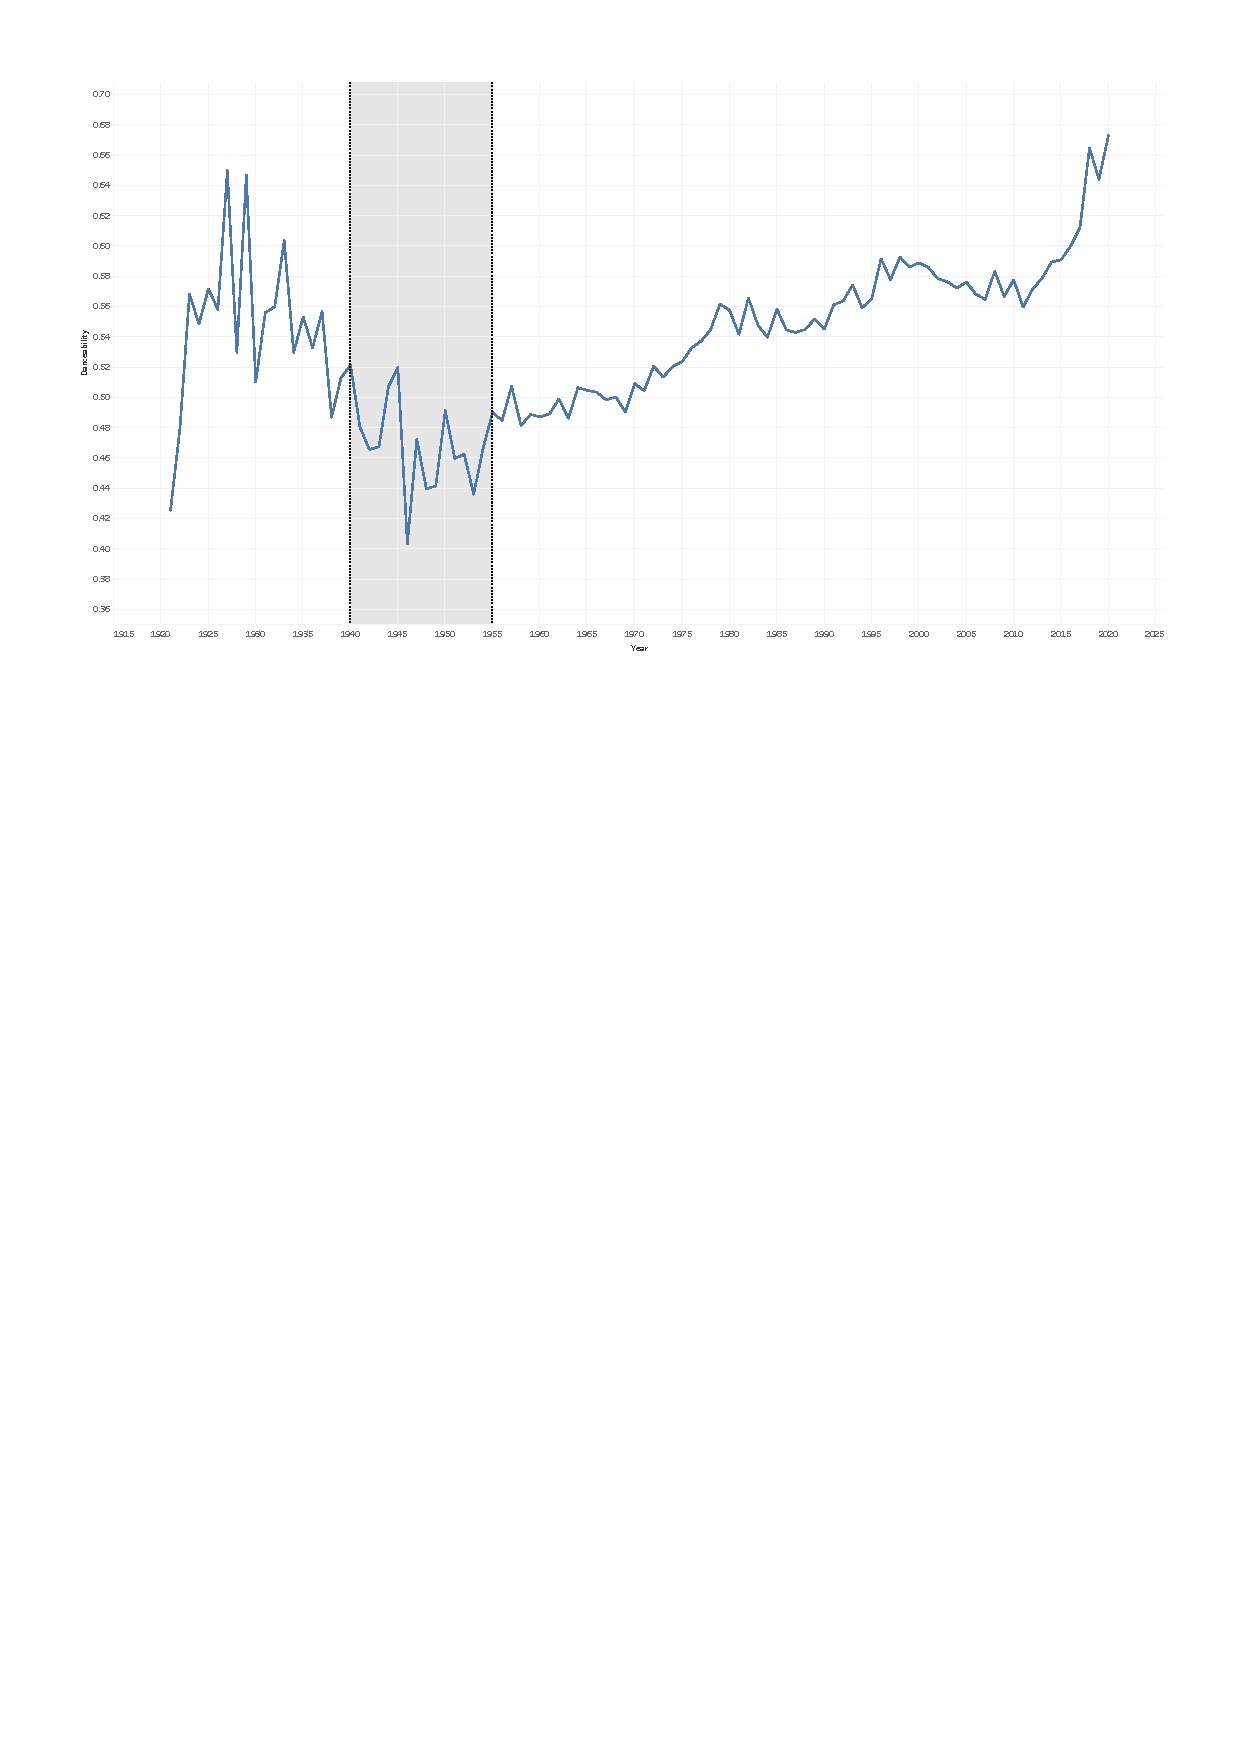
\includegraphics[width=0.4\textwidth]{qushi3.pdf}}			  % 子图1的相对位置
		\subfigure[Valence]{				% 图片2
			\label{Fig.sub.match4}						% 子图2的标签
			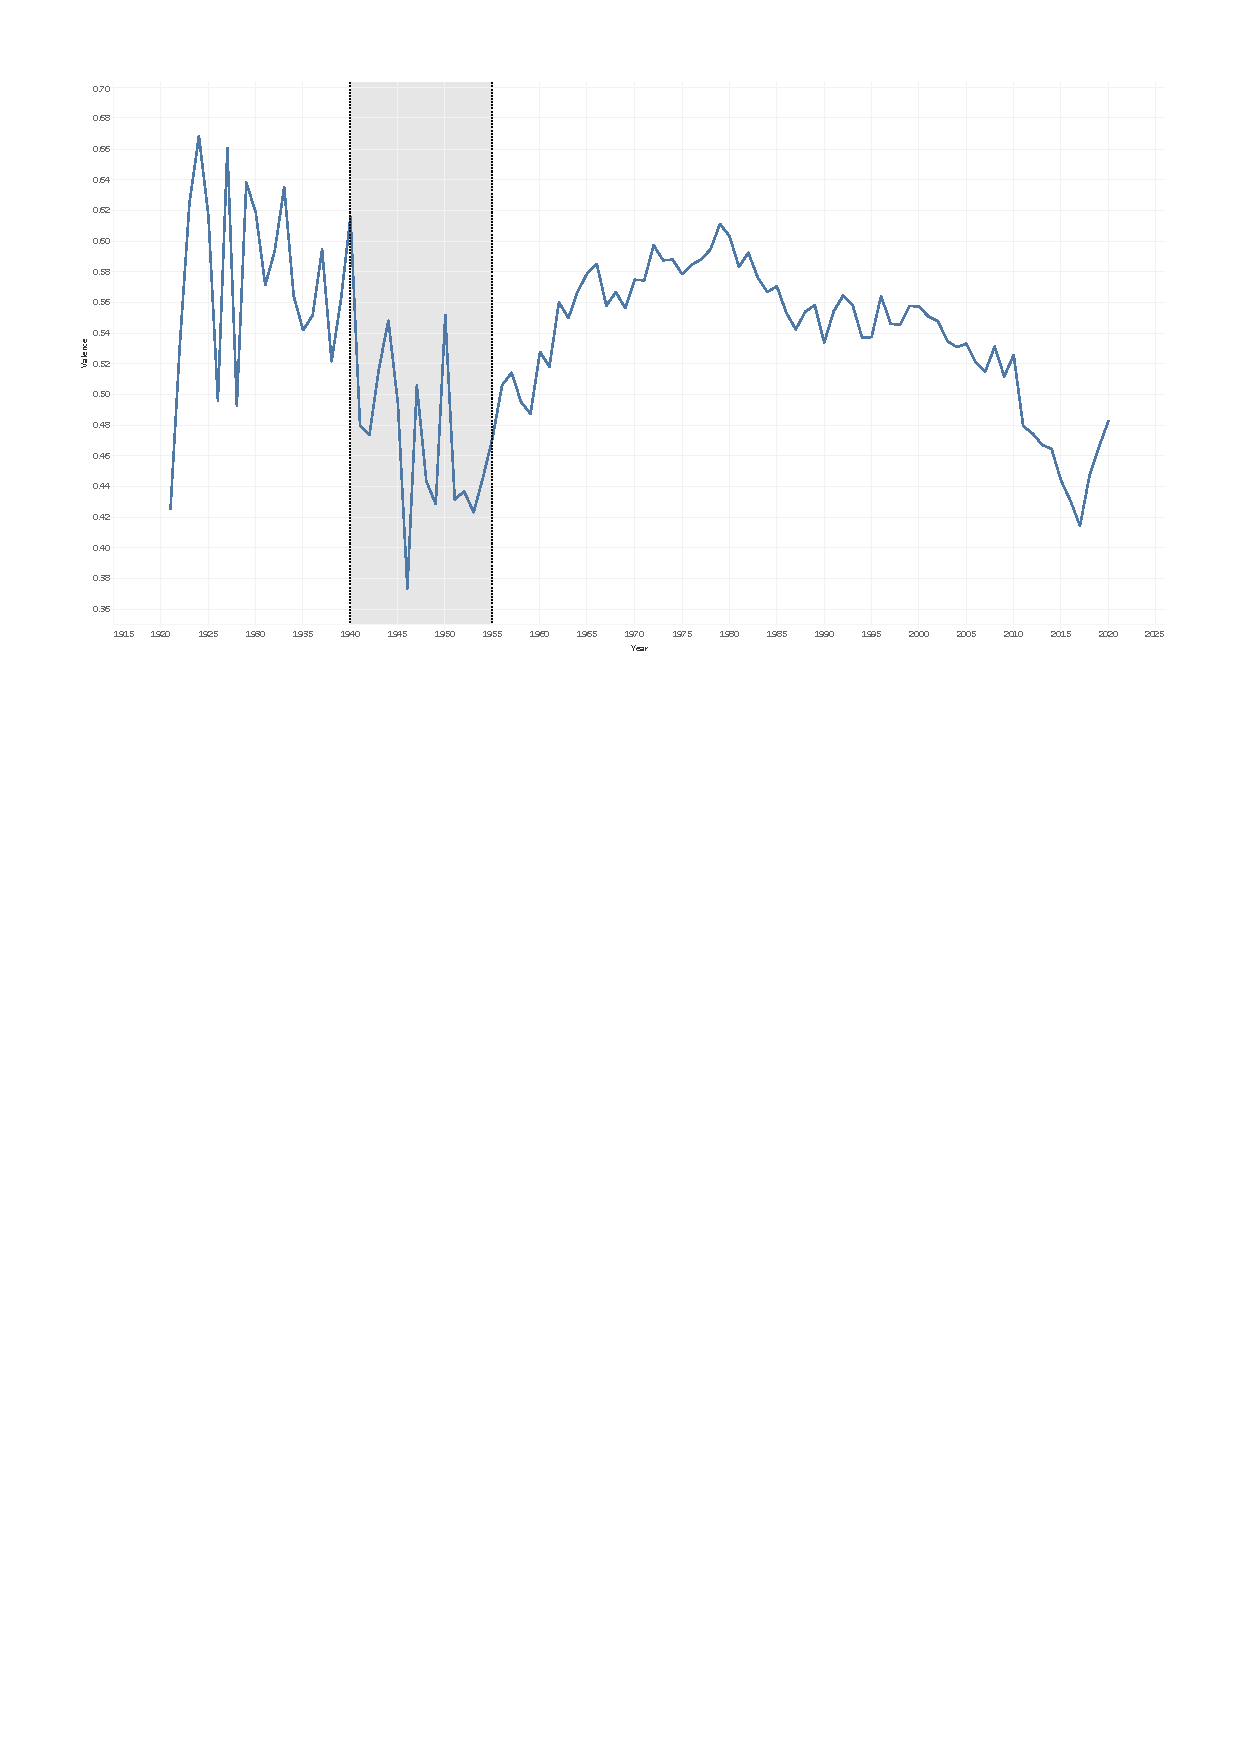
\includegraphics[width=0.4\textwidth]{qushi4.pdf}}
		\caption{Culture-influence processes}		% 总图标题
		\label{Fig:cip}									% 总图标签
	\end{figure}
	
	\textbf{Period I (1935-1945):} This Period was shaped by the moods of the Great Depression. In
	these period, lots of artists begin to create music with high energy and fast tempo, as shown in
	Figure 17. Reinvention and fast growth of Pop/Rock and the glamorous beginning of Reggae
	form an upward look of culture.
	
	\textbf{Period II (1950-1960):} Following the detrimental effects of World War II, people was about
	to embark on a musical journey and substantially change the music style, valence and danceability saw a sharp increase in music released in this period – the golden age of Pop/Rock. The
	whole culture becomes hopeful and energetic.
	
	\textbf{Period III (1995-2005):} By late 1995, many young people were getting tired of the Pop/rock
	were inundating the airwaves with, the energy and tempo of music reached the peak and began
	to decline. A mature music culture is gradually formed
	
	\subsection{Changes identified within the network}
	
	\textbf{Social and Political Changes:} According to Similarity Network of Pop/Rock
	artists in 1950s. As shown in figure 18, 1950s’ Pop/Rock is diversified in several subgenres,
	which are rather different from each other (as there are no edges between artists in different
	subgenres). This feature of network identifies the countercultural movement in 1950s – people
	have increasing desire for true freedom of expression and the diversity of people become more
	and more prominent.
	
	\textbf{Technological Changes:} According to the Wikipedia, we know that the emergence of the
	Internet mainly leads to the rise of the Electronic, as the Internet made it easier to spread the
	software for producing Electronic music. Such trends can be identified through change of numbers of influencers in Electronic over time, as shown in figure 19. Influence reaches its peak
	due to the proliferation of the Internet.
	
	Analysis above shows that based the models established, we can find the cultural influence
	of music in time and circumstances, and identify the effects of social, political or technological
	changes. 
	
	\begin{figure}[htbp]
		\centering
		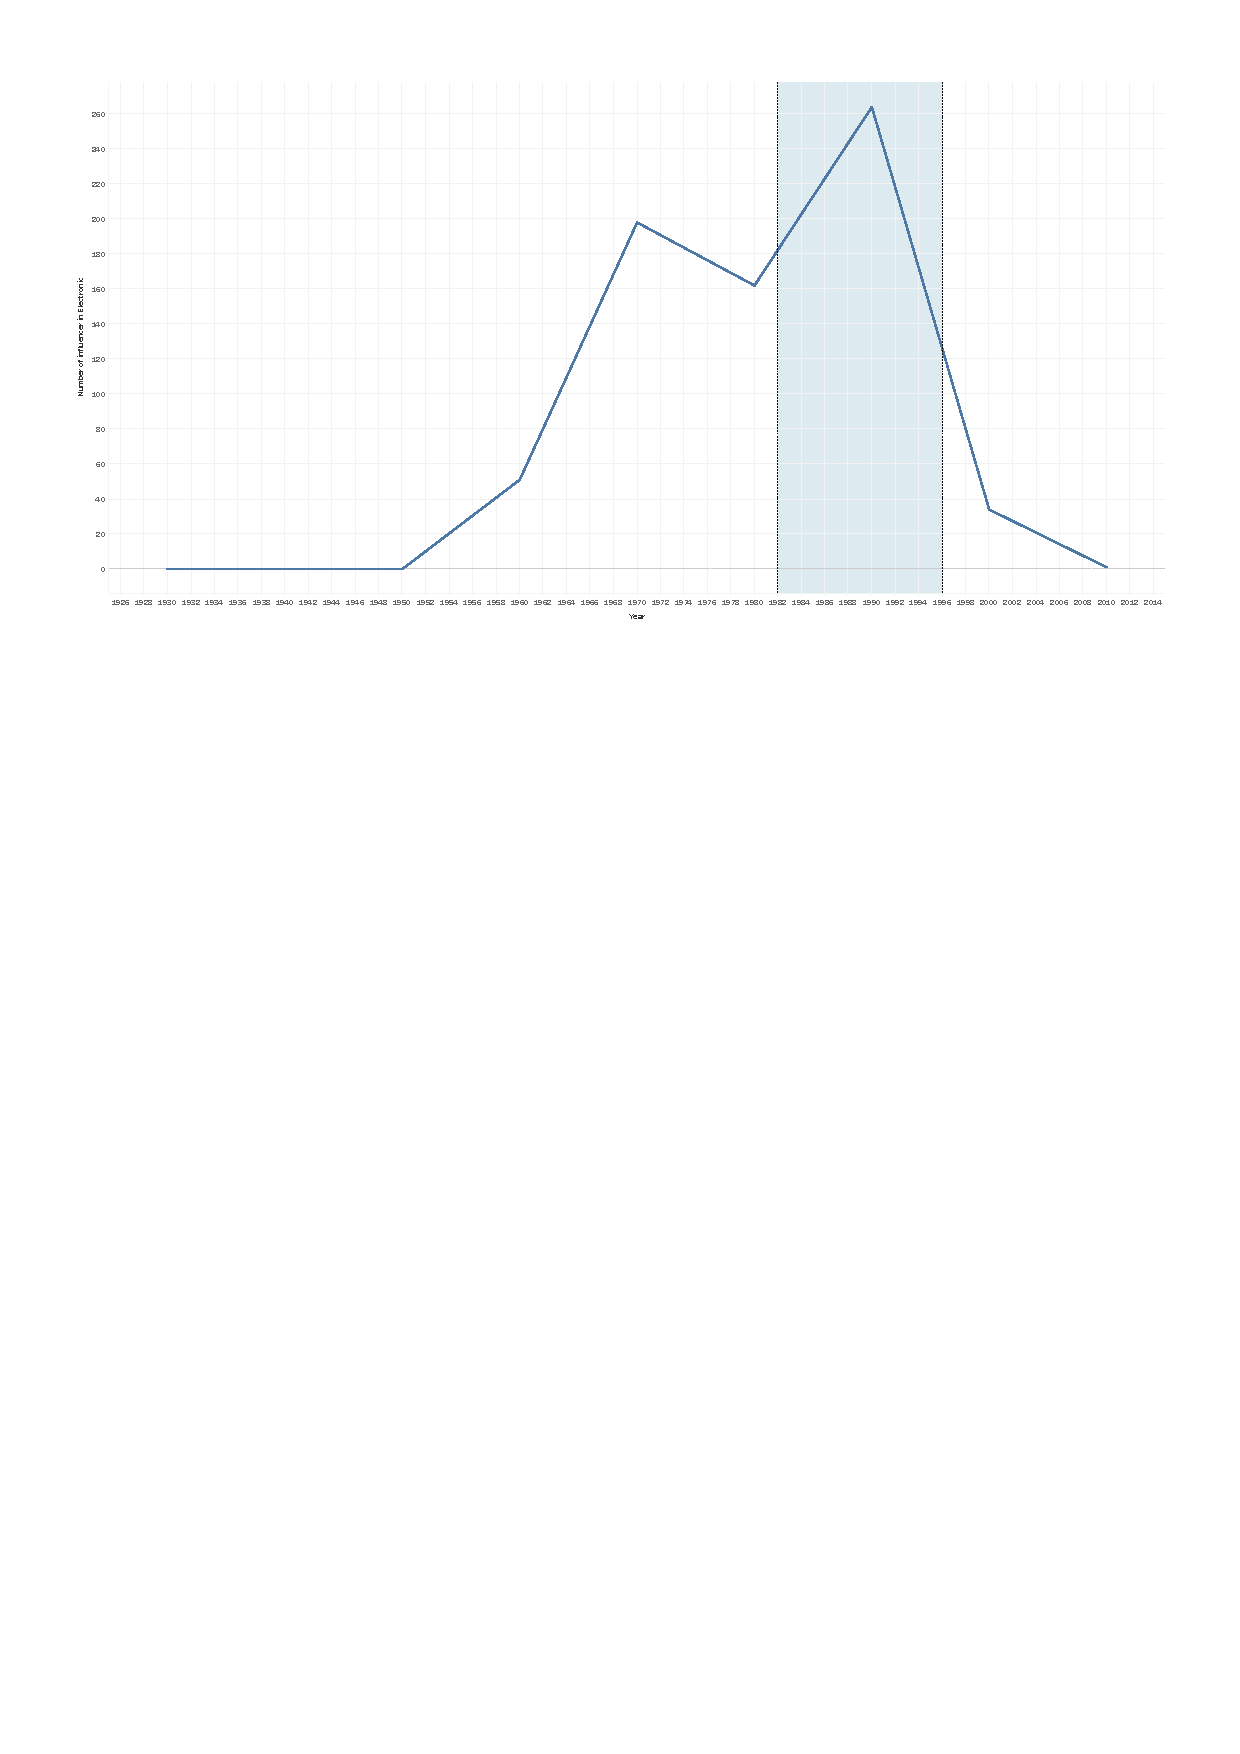
\includegraphics[width=1\textwidth]{elc.pdf} 	% 图片相对位置
		\caption{Number of influencers in Electronic}		% 图片标题 
		\label{fig:inelc}							% 图片标签
	\end{figure}
	
	
	\section{Analysis on Model's Sensitivity}
	
	In \textsc{Task 5}, our Change Point Detection model involves a trimming parameter $ \tau $, which might have an effect on optimal change points detection. To test the robustness of the model, we apply a change to the trimming parameter and check whether the revolutionary in 1950s can be well detected.
	
	\begin{table}[!htbp]
		\begin{center}
			\caption{Influence of $ \tau $ on change point detection}
			\begin{tabular}{ccccc}
				\toprule
				\multicolumn{5}{c}{$\tau$} \\
				\cline{2-5}
				Characteristic  & {[0.05n]} & {[0.10n]} & {[0.15n]} & {[0.20n]} \\
				\midrule[1pt]
				\text { Acousticness } & 195019641979 & 195019641979 & 195019641979 & 195019641979 \\
				\text { Danceability } & 1928195119972008 & 195019972008 & 195019972008 & 19502008 \\
				\text { Energy } & 1951198319942008 & 195119792008 & 195119792008 & 195119792008 \\
				\text { Loudness } & 1936195119802008 & 193619502008 & 193519502008 & 19502008 \\	
				\bottomrule
			\end{tabular}\label{tb:infcpd}
		\end{center}
	\end{table}
	
	As shown in \textbf{Table \ref{tb:infcpd}}, the proposed model is very robust to change points when $ \tau $ is greater than or equal to [0.1n], which implies the value we selected is reasonable.
	
	
	\section{Strengths and Weaknesses}
	\subsection{Strengths}
	\begin{itemize}
		\setlength{\parsep}{2ex} %段落间距
		\setlength{\topsep}{2ex} %列表到上下文的垂直距离
		\setlength{\itemsep}{1ex} %条目间距
		\item \textbf{Effective models:} For different problems, we build several models including Similarity network, Change Point Detection model, which makes the analysis of each problem detailed and convincing.
		\item \textbf{Statistical tests:} Instead of simply comparing the value, we apply Mann-Whitney Test and Multivariate Mean Test to make our conclusions are reliable.
		\item \textbf{Vivid visualizations:} We use many figures to show our results, make it easier to capture the key information.
	\end{itemize}
	\subsection{Weaknesses}
	\begin{itemize}
		\setlength{\parsep}{2ex} %段落间距
		\setlength{\topsep}{2ex} %列表到上下文的垂直距离
		\setlength{\itemsep}{1ex} %条目间距
		\item Our analysis does not cover all genres in some models. Given space limitations, part of our analysis mainly focuses on two representive genres: Pop Rock and R\&B.
		\item We make a strong assumption on time series, which doen’t always hold in reality. We assume the error term follows independent normal distribution, however, it often follows a weakly dependent stationary process in reality.
	\end{itemize}
	
	
	% \section{Model Promotion}
	% The model can be extended to many industries, such as the courier industry, the medical industry, the retail industry.
	% Take the courier industry as an example, we can compare a courier point to a charging station. Courier service range corresponds to the mileage of the electric car after charging, while the average delivery time corresponds to the average waiting time for electric car charging. Moreover, the demand for expressing delivery is very different in cities, suburbs and villages. Therefore, it is completely possible to use the charging station model to distribute the courier points.
	
	% \section{Conclusion}
	% \begin{itemize}
		%     \item In the future, it is very likely that among the majority of countries, electric vehicles will be completely popularized. Besides, the stagnation of the rest countries could be attributed to their own geographical reasons, such as Indonesia, Venice and other countries or regions.
		% \item The main influencing factors which trigger different modes of network growth contain the density of population, the distribution of wealth, the strength of science and technology and cost. Besides, different factors may cause different effects.
		% \item The cost has a great influence on the development of the charging station network, while the population density has only a slight impact.
		% \end{itemize}
	
	
	
	% 参考文献,此处以 MLA 引用格式为例
	\clearpage
	
	\section{A Document to ICM Society}
	
	\leftline{\textbf{To}: Integrative Collective Music Society}
	
	\vspace{-1mm}
	
	\leftline{\textbf{From}: Team 048}
	
	
	We are proud to inform you of the results of our data analysis, following the creation of a model for the evaluation of musical influence and similarity.
	
	Our team has modeled the interactions between and within musicians across genres from 1921 to 2020. We built a directed network to analyze the interactions between musicians and to understand the interactions that exist between musicians. An evaluation model to measure the similarity between music was developed to provide an evaluation of the similarity between and within genres and to give the distinctive features of music in each genre. An evaluation model based on a sliding window was developed to select the leading figures of each genre in different time periods.
	
	With the model we developed, we obtained the following valuable conclusions.
	
	The influence among musicians is in accordance with Pareto's Principle, which states that a very small number of musicians have influenced the vast majority of musicians. We can assume that a very small number of outstanding musicians led the way for the entire musical community, and an in-depth exploration of the works of these musicians may deepen our understanding of the music.
	
	The music of each genre is not completely independent of each other, but rather intermingles without clear boundaries. As a vehicle for human emotion, there are similarities between genres of music. Studying the alternating fusion and evolution of music among genres is conducive to enhancing our perception of the evolution of music as a whole.
	
	The changes in music can clearly reflect the changes in society. Music is a tool for people to express their feelings, and by monitoring the changes in musical emotions, we can probe the pent-up emotions in society and thus make predictions about social change. Policy makers can try to adjust their policies accordingly by responding to the emotions expressed in current music.
	The model we have built is still limited by the incomplete data and the space limitation. We need more data for the following purposes.
	
	We found that some of the singers are non-common in both datasets, and the debut time of some of the singers is also unknown, which creates some inaccuracy in our analysis. We would like to obtain a more complete dataset of artists and music.
	
	If we know the specific year in which the influenced person was influenced by the influencer, then we can refine the model to determine the contagion of the music and whether the change was actually made by the influencer's music before and after the year of influence. Also the dynamic influence index of the influencer can be refined based on the change in the number of influenced people.If we know the information about the album the song is on, then we can modify our model to capture the short-term impact by directly comparing the similarity between albums.
	
	We hope in the future to build a dynamic network in the time and genre dimensions. We also hope to make a more detailed segmentation in genre and develop a visualization system to more clearly depict the intrinsic development. These are the results of our team's work We sincerely hope to provide you with useful information and data.
	
	\clearpage
	
	\begin{thebibliography}{99}
		\bibitem{1} Chen, Guanrong. Introduction to complex networks : Models, structures and dynamics [M]. Higher Education Press, 2012.
		\bibitem{2} Lawley D N . A GENERALIZATION OF FISHER'S z TEST[J]. Biometrika, 1938, 30(1-2):180-187.
		\bibitem{3} Rencher A C . Methods of Multivariate Analysis[M]. John Wiley \& Sons, Inc, 1995.
		\bibitem{4} Mcknight P E , Najab J . Mann-Whitney U Test[M]. John Wiley \& Sons, Inc. 2010.
		\bibitem{5} Jushan, Bai, Pierre,et al. Computation and analysis of multiple structural change models[J]. Journal of Applied Econometrics, 2003.
	\end{thebibliography}
	
	
	
	
	
	
\end{document}  % 结束